\documentclass[12pt]{article}

% TEMPLATE DEFAULT PACKAGES
\usepackage{amssymb,amsmath,amsfonts,eurosym,geometry,ulem,graphicx,color,setspace,sectsty,comment,natbib,pdflscape,array,adjustbox,threeparttable}

% ADDED PACKAGES FOR THIS MANUSCRIPT
\usepackage{palatino,newtxmath,multirow,titlesec,threeparttable,tabu,booktabs,titlesec,threeparttable,mathtools,bm,bbm,subcaption,pdflscape,tcolorbox,mathrsfs,float}
% endfloat,

%\usepackage{kbordermatrix}% http://www.hss.caltech.edu/~kcb/TeX/kbordermatrix.sty
%\usepackage{amsmath}% http://ctan.org/pkg/amsmath

\usepackage[colorinlistoftodos]{todonotes}

\usepackage{afterpage}
\usepackage[hyphens]{url}
\usepackage[margin=1cm]{caption}

\usepackage[draft]{hyperref}
\newcommand{\tim}{$\,\times\,$}
% FIGURES & TABLES CAPTION STYLING
\captionsetup[figure]{labelfont={bf},name={Figure},labelsep=period}
\captionsetup[table]{labelfont={bf},name={Table},labelsep=period}

% SECTION TITLE SETTINGS
\titlelabel{\thetitle.\enskip}
\titleformat*{\section}{\large\bfseries}
\titleformat*{\subsection}{\normalsize\bfseries}

% COLUMN TYPES
\newcolumntype{L}[1]{>{\raggedright\let\newline\\\arraybackslash\hspace{0pt}}m{#1}}
\newcolumntype{C}{>{\centering\arraybackslash}p{5.2em}}
\newcolumntype{D}{>{\centering\arraybackslash}p{5em}}
\newcolumntype{E}{>{\centering\arraybackslash}p{6em}}
\newcolumntype{R}[1]{>{\raggedleft\let\newline\\\arraybackslash\hspace{0pt}}m{#1}}


% MARGINS AND SPACING
\normalem
\geometry{left=1.1in,right=1.1in,top=1.0in,bottom=1.0in}
\setlength{\parskip}{2.5pt}

% SPECIAL CELL 
\newcommand{\specialcell}[2][c]{%
	\begin{tabular}[#1]{@{}l@{}}#2\end{tabular}}

% NO INDENT ON FOOTNOTES
\usepackage[hang,flushmargin]{footmisc}

\begin{document}

\begin{titlepage} 
%\title{{Borrowing with Unpaid Bills}\thanks{}}
\title{{Microcredit from Delayed Bill Payments}}
\author{\\[3em]
  William Violette\thanks{Federal Trade Commission, Washington, DC. E-mail: william.j.violette@gmail.com   Any opinions and conclusions expressed herein are those of the author and do not necessarily represent the views of the Federal Trade Commission or its Commissioners.} \\
 \\ 
  }
\vspace{30mm}
\date{\vspace{5mm}This Version: \today}
\maketitle
\begin{abstract}


Delaying bill payments to public utilities may provide an important source of credit to households.  With billing data from a water utility in Manila, Philippines, this paper builds a consumption and savings model to estimate demand for both water and credit.  Estimates suggest that households value billing flexibility\todo[color=green]{What kind of flexibility, temporal?} \todo[color=red]{A does this mean being able to not pay? under what terms?} from the water utility as much as 8
\unskip\% of an average water bill.  I then analyze the welfare effects of popular proposals to reduce delinquency by requiring upfront payments.  Simulations find that upfront payments do not produce enough cost savings \todo[color=red]{A to whom?} to justify their negative impacts on household consumption smoothing.\todo[color=green]{``Recoup less revenue then it would take to compensate for their loss of consumption smoothing''}


\vspace{2in}
\textbf{Keywords:} credit constraints; consumption smoothing; water utilities. \\
\textbf{JEL Codes:} O13; E21; L95. \\
\bigskip
\end{abstract}
\setcounter{page}{0}
\thispagestyle{empty}
\end{titlepage}
\pagebreak \newpage

%\spacing{1.5}
\onehalfspacing

\section{Introduction}

Households face a dynamic problem of how to smooth their consumption over time, especially in low-income settings where households have little access to formal credit and risky income streams (\cite{morduch1995income}).  Households often resort to costly money lenders or informal arrangements with family members (\cite{banerjee2007economic}).  Firms may provide an additional channel for consumption smoothing by allowing households to delay their payments for goods and services.  In particular, public utilities often tolerate high levels of delinquent bills each month.  Delinquent bills provide an economically important source of credit for households since public utilities cover broad populations and take up at least \todo[color=red]{A approximately?} 5\% of household incomes in developing countries.\footnote{\cite{komives2006distributional} find that households spend 1-2\% of their incomes on water and 4\% on electricity.} 

When market failures limit formal lending, public utilities may provide efficient, second-best sources of credit.\todo[color=red]{A second best to whom? maybe add a footnote?}  First, poor access to collateral often restricts the availability of \todo[color=red]{A formal?} lending options to low-income households (\cite{jack2016borrowing}).  Public utilities overcome this barrier by threatening disconnection from future service to enforce repayment.  Second, poor infrastructure and mobile populations increase the transaction costs of screening and monitoring debtors, which contribute to high interest rates (\cite{jack2014risk}).  As part of their business practices, public utilities invest in meter reading and billing systems that may lower these transaction costs.  Third, moneylenders and peer-to-peer lending groups often cater to small pools of debtors while public utilities are able to spread default risk across a wide customer base.  Despite these advantages, linking credit to consumption from public utilities creates an inherent inefficiency by incentivizing overconsumption.  For example, households may substitute toward piped water and away from other beverages in months where they are credit constrained.\todo[color=red]{A absent externalities from water consumption? mention in footnote}\todo[color=green]{This seems so minimal, do you know if hh sell water when credit constrained or other direct evidence?  I need a more compelling example of overconsumption. A: wash clothes at home or outside the home}  Since governments actively regulate public utilities, the extent to which public utilities \todo[color=red]{A maybe whether or not is a better way to frame it}should provide credit remains an open policy question (\cite{laffont2005regulation}).  \todo[color=red]{A both of water/electricity and other stuff through credit? i'm just saying that even without the credit story, forcing you to pay would make you lose from not smoothing your water consumption. and then with credit, you also lose from not smoothing other stuff, right?}

Technologies that eliminate delayed payments have recently dominated utility policy discussions.    Both researchers and policymakers recommend new prepaid metering technologies, which require upfront payments before releasing any services, as effective strategies to prevent nonpayment.\footnote{\cite{kojima2016making} and \cite{heymans2014limits} point to prepaid metering as a successful strategy to reduce nonpayment for electricity and water utilities (respectively).  \cite{jack2016charging} find that prepaid meters for electricity in South Africa substantially increase utility revenues.}    Yet, existing analyses have yet to consider how these technologies may impact household welfare by reducing consumption smoothing.

This paper incorporates delayed payments to public utilities into household consumption and savings decisions in order to evaluate the welfare effects of offering credit through public utilities.  I build a dynamic model where each period, households have the option of borrowing with a costly asset as well as with delayed payments to a public utility.  Low interest rates on delayed payments induce households to increase their borrowing by overconsuming utility services.\todo[color=red]{A so there's 2 things going on here, right? 
1. i get credit by not paying my bill on my fixed consumption c
2. more credit by not paying and consuming c'>c cause it's cheaper than buying other beverages }  The extent to which households value payment flexibility depends on the borrowing costs of other assets, which are often difficult to measure in traditional survey data. \todo[color=red]{A  i'm still having trouble here. is this just the option of not paying? but what's the risk? what are the terms of this "loan"? how long can i do it? etc. 
i think i get what you're saying but i'm hung up on how this may be different in many scenarios. for example, in mex it's illegal to cut off people's water supply. so if they don't pay, i think the most you can do is decrease their flow or something}

\todo[color=red]{A formal or utilities?
oh ok. borrowing costs from i guess formal lenders and also roscas and all those informal ones}To estimate borrowing costs, I take a structural approach using billing data from a regulated water utility in Manila, Philippines.  The identification strategy leverages months where utility workers visit households and disconnect them if they do not pay their outstanding balances.  If borrowing were costless, households would never be disconnected during these visits because they would pay their outstanding balances with cheap loans.  Therefore, long and frequent disconnections in response to these visits --- especially among households with large outstanding balances --- provide evidence of borrowing costs.\todo[color=green]{Or they have a cheap alternative source of water?} \todo[color=red]{A any alternative explanations?
for example, what if this is just substitution? it's not that borrowing money is expensive, it's just that i won't pay and get water from my neighbors or a vendor. }  Using this strategy, I estimate high interest rates for borrowing, consistent with poor observed access to formal credit in Manila with only 3.9\% of households having credit cards and 18.7\% having bank accounts.\footnote{Statistics are from the Philippines 2014 Consumer Finance Survey.}  \todo[color=green]{Compare to actual interest rates here}

These estimates also allow me to simulate several counterfactual policies.  First, I find that in a counterfactual where households are required to pay their bills on time (holding all else equal), consumer welfare drops by 50.3
PhP (or 1.5
USD) per household-month, which is equal to 8
\unskip\% of an average water bill.\todo[color=orange]{D How much of household consumption?}  Usage also declines since households no longer have an incentive to overconsume water to fund their borrowing from delaying bill payments.  

Second, I simulate a policy that (1) eliminates delayed payments by charging a high interest rate on unpaid bills, (2) eliminates default risk by preventing households from leaving large outstanding balances when they permanently disconnect, and (3) adjusts prices to ensure that the water utility remains revenue-neutral (consistent with regulation in Manila).\footnote{\cite{laffont2005regulation} discusses economic reasons for these regulatory structures which are common in both developed and developing country settings.}  Without default risk, the utility has fewer costs to recover with prices. Yet without billing flexibility, households use less water, generating less revenue for the utility.  On net, prices remain the same and the policy reduces social welfare by 89.4
PhP (or 2.0
USD) per household-month.  

Finally, I use this framework to evaluate implementing prepaid meters in this context.  While ensuring that households pay upfront, prepaid meters require steep increases in prices to cover their installation and maintenance costs.  As a result, prepaid meters produce large reductions in social welfare on the order of 245.5
PhP (or 5.0
USD) per household-month.  Taken together, these results suggest that popular policies to reduce nonpayment may be welfare reducing primarily by limiting consumption smoothing.\todo[color=green]{ Decompose loss due to cost and due to consumption smoothing? }  Given around 2.4 million piped water using households in Metro Manila, these policies would imply welfare costs on the order of 32.7
to 144.1
million US dollars per year. \todo[color=orange]{D how many are affected by law? }

This paper contributes to three main strands of economic literature.  First, this paper brings payment and billing policy questions into a growing literature on optimal policy for utilities in developing countries (\cite{mcrae2015infrastructure}; \cite{szabo2015value}; \cite{jack2016charging}; \cite{jack2015pay}; \cite{szabo2015reducing}).  Building on previous static models, this paper also provides a framework for considering how dynamic incentives affect household demand for public utilities.  Second, this paper draws on a large body of research analyzing household credit constraints, particularly through microfinance interventions (\cite{morduch1999microfinance}; \cite{morduch1995income}; \cite{cull2009microfinance}; \cite{dupas2013savings}; \cite{jack2016borrowing}).  \cite{karlan2009expanding} and \cite{gine2014group} specifically focus on microfinance in the Philippines. Third, \cite{deaton1991saving} provides the foundational model of dynamic decision-making that serves as the starting point for the model in this paper, and the estimation of this model adapts methods developed by \cite{gourinchas2002consumption} and \cite{laibson2007estimating}.

This paper proceeds with Section~\ref{section:data} describing the water billing data from Manila.  Billing practices, disconnection policies, and institutional details are discussed in Section~\ref{section:descriptives} alongside descriptive evidence.  Section~\ref{section:model} develops a model of household consumption and savings decisions while Section~\ref{section:estimation} discusses the estimation and results.  Counterfactual exercises and welfare impacts are provided in Section~\ref{section:counterfactuals}.  Section~\ref{section:conclusion} concludes. \todo[color=orange]{ non-pay correlated with other non-pay? possibility of bribery?}

\section{Data}\label{section:data}

% Describe notice of disconnection in more detail here??? and  NO DO IT LATER~! PLEASE!!!!

Measuring creditab wt through delayed water bill payments requires information on water consumption and bill payments at the household-level as well as features of the credit environment in Manila.  % As well as information on the credit environment facing households

Water consumption and bill payments come from water utility records collected as part of a research partnership with one of the two regulated utilities in Metro Manila, Philippines where each utility is responsible for serving their assigned geographic half of Metro Manila.  This utility provided access to monthly billing records for each connection as well as detailed information covering the regulatory structure and costs of production.  Monthly billing records include meter readings, billing amount, outstanding balances, and payments spanning January, 2008 to May, 2015. 

Disconnection is defined as months with missing values for usage.  Months with zero recorded consumption are not considered disconnected.  Since households face a 200 PhP reconnection charge but a 


Over this period, the total number of connections increased from 900,000 to 1,500,000 as the water utility expanded service access.  Water connections are split into four categories: residential (90\%), semi-business (4\%), commercial (5\%), and industrial (1\%).  

To examine household demographics, connections are linked to a water connection survey conducted independently to monitor the quality of the utility's service.  The survey randomly interviewed households with water connections covering 15,000 households in 2008, 24,000 households in 2010, and 23,000 households in 2012.  Since the survey followed a similar sampling design across rounds, 13\% of households were interviewed in two waves and 1.4\% of households were interviewed in three waves while remaining households were interviewed in one wave.  To focus on household decisions, the analysis includes only residential connections that are identified in this survey as serving a single household (31\% of all connections).  The connection survey also includes demographics for households that own their water connections.  Households using connections alone tend to be larger and wealthier than households that share connections with other households according to previous research (\cite{wjv}).  Table~\ref{table:sampleconstruction} in Appendix~\ref{appendix:sampleconstruction} includes more details on how the final sample is constructed for the analysis.
% This sample restriction ensures that connection-level is equal to household-level.

DESCRIBE CBMS!

Since the analysis focuses on the borrowing and savings behavior of a representative household, additional data sources help characterize credit access in Manila.  Average household income is calculated using the  2015 Family Income and Expenditure Survey, which covers 4,130 households in Metro Manila.  Interest rates for borrowing and saving come from the 2014 Consumer Finance Survey in Metro Manila as well as the World Bank Databank (2010-2015) for the Philippines.  



% To exclude connection-level survey data, which measure the number of households using each connection as well as demographics for the household that owns the connection.  Conducted every two years between 2008 and 2012, the survey covers a cross-section of nearly 50,000 water connections.  Documentation indicates that surveyors used stratified random sampling where the number of connections surveyed was proportional to the census population in the smallest administrative census region, making this survey roughly representative of the population of piped water users.  To examine the consumption and savings behavior of individual households, the analysis is limited to surveyed connections that serve only one household (31\% of surveyed connections), which tend to serve larger, wealthier households according to previous research (\cite{wjv}).  This sample restriction also ensures that connection-level is equal to household-level.

% Measuring household income for water users requires two-steps: in the first step, billing data are merged with connection-level survey data on household demographics.  In the second step, household income is imputed with household location and demographics using additional survey data on household income.

% The first step uses connection-level survey data, which measure the number of households using each connection as well as demographics for the household that owns the connection.  Conducted every two years between 2008 and 2012, the survey covers a cross-section of nearly 50,000 water connections.  Documentation indicates that surveyors used stratified random sampling where the number of connections surveyed was proportional to the census population in the smallest administrative census region, making this survey roughly representative of the population of piped water users.  To examine the consumption and savings behavior of individual households, the analysis is limited to surveyed connections that serve only one household (31\% of surveyed connections), which tend to serve larger, wealthier households according to previous research (\cite{wjv}).  This sample restriction also ensures that connection-level is equal to household-level.




% Since multiple households often share the same connections in Manila, 



% The second step leverages the 2015 Family Income and Expenditure Survey, which covers 2,528 households across 216 wards that overlap with the connection survey.  This cross-sectional survey collects detailed information on household income, demographics, and measures of credit usage.  The analysis is further limited to data from these 216 geographic wards (18\% of wards covered by the connection-level survey).\footnote{Wards in the Philippines are known as ``Barangays,'' and have average populations of 7,600 people in Metro Manila.}  Income is imputed with a linear regression of indicators for each household size, each number of employed household members, each age of household head, each ward, and each dwelling type (duplex, single-house, and apartment).  Log-income is used for imputation both to prevent negative values for imputed incomes and to match the right-skewed distribution of household income.\footnote{The imputation procedure results in an $\text{R}^{2}$ of 0.48.}  



% Since the distribution of household income  and ensure that imputed incomes are positive.
% To impute household income, 

% Since connection survey data do not include income measures, household income is imputed from household survey data according to demographics and location.  The household survey data 


% Household income is imputed using household demographics and location from connection-level survey data and separate household survey data.  

% The billing data is merged at the water connection level to survey data that measures the number of households using each connection as well as demographics for the household that owns the connection.  Conducted every two years between 2008 and 2012, the survey data cover a total of nearly 50,000 water connections.  Connection survey documentation indicates that surveyors used stratified random sampling where the number of connections surveyed was proportional to the census population in the smallest administrative census region, making this survey roughly representative of the population of piped water users.  

% To analyze consumption and savings decisions at the household level,  
% The analysis focuses on 

% the analysis is further limited to connections that each serve a single household in order to ensure that billing data for each connection maps directly into the consumption and savings decisions of a single household.\todo[color=green]{Its not clear from identification strategy that I need to drop them, too much detail, just do generalizability sentence at the end.}  

% Previous research from \cite{wjv} finds that sharing a connection with multiple households increases the costs of consuming water for each household, which affects each household's water demand.  \cite{wjv} also finds that households using a connection individually tend to have higher water demand, larger household sizes, and greater likelihood of living in single houses (as opposed to duplexes or apartments) in comparison to households sharing water connections.  These differences may limit the generalizability of the findings outside of this subpopulation in Manila.  

% This sample restriction also ensures that household-level data and connection-level data\todo[color=green]{Do you know if its the same HH over time? (no, but make that clear!)} can be referred to interchangeably.  Table~\ref{table:sampleconstruction} in Appendix~\ref{appendix:sampleconstruction} includes more details on how the sample is constructed for the analysis. 

% Because the connection survey data does not include income measures, average monthly income for households in Manila is taken from the 2015 Family Income and Expenditure Survey.  

% % Mention later: average interest rate, and other calibrations 
% % The average interest rate for the Philippines is calibrated from the World Bank Databank (2010-2015).


\section{Credit through Delayed Water Bill Payments}\label{section:descriptives}

% \footnote{The company upgraded t in the first year of the sample.  Previously, the company mailed the bill to each household at the end of the month.} 
% Each month, households consume 24m3 of piped water on average, which totals an average monthly bill of 691.6PhP as shown in Table~\ref{table:descriptives_all}.  Given an average monthly income in Manila of 31,910PhP and savings rate of 5,730PhP,  monthly water bills reach a modest average of 2.2\unskip\% of income and 10.6\unskip\% of savings.  

%%% NOTES FROM TOWNSEND PAPER ! %%%
% For the purposes of this partial equilibrium analysis, this borrowing constraint is exogenous.
% It is not a natural borrowing constraint as in Aiyagari (1994) and therefore somewhat ad
% hoc, but such a constraint can arise endogenously in models with limited commitment (see
% Wright (2002)) or where lenders have rights to garnish a fraction of future wages (e.g.,
% Lochner and Monge-Naranjo (2008))

In Manila, households have poor access to credit.  Small-scale loans mainly from money lenders and micro-finance groups are the most common forms of credit and charge high monthly interest rates of 9.5\unskip\% on average.\footnote{According to the 2014 Consumer Finance Survey in Manila, 1\% have credit cards, 3.8\% have auto-loans, 0.5\% have mortgages, and 12\unskip\% have all-purpose loans, of which 61\unskip\% are from money lenders and 15\unskip\% are from micro-finance groups.}  In this environment, delaying water bill payments may provide a reliable, alternative source of credit because the water utility often tolerates high rates of delinquency before disconnecting water service and the utility is prohibited from charging any interest on outstanding balances.  

Households often delay their water bills.  Instead of paying each month, households make large, infrequent payments.  Table~\ref{table:descriptives_all} provides summary statistics on household consumption, billing, and payments.  While the average bill is 691.6PhP per month, payments average 901PhP, occur in 61\unskip\% of months, and leave households 50days behind on their bills.  Each month, the average household maintains 2,068PhP in unpaid water bills and only 538 PhP in small-scale loans mainly from money lenders and micro-finance groups.\footnote{According to the 2014 Consumer Finance Survey in Manila, 12\% of households have small-scale loans.  Average loan sizes equal 51,280PhP with an average period of 9months.}   With average monthly incomes of 31,910PhP, households spend around 3\% of their income on water while unpaid water bills total around 5.5\% of their income.\footnote{For reference, 1 USD is worth around 45 PhP over this period.}   
% those that are at least two months delinquent

The utility enforces payment by visiting households and disconnecting them if they do not immediately pay their bills.\footnote{Disconnection typically involves placing a metal lock on the water meter that stops any flow.}  While households often try to negotiate for additional time to pay their bills, 96\unskip\% of households report having to pay within 30 days and the average grace period is only 13days.  As a result, only 25\unskip\% of households report having ``enough time'' to make their payments, which may be in part due to poor credit access in Manila.  While disconnected, households likely substitute to alternative water sources including sharing with neighbors, using from deepwells, or purchasing from local water vendors.  In the 2012 wave of the water connection survey, 6.1\unskip\% of households report having been disconnected for delinquency.  The billing data find that even among households that remain connected at the end of the sample period, 2\% of their months are spent temporarily disconnected on average.  To reconnect, households must pay any outstanding bills as well as 200 PhP reconnection fee.

The utility must frequently enforce payments because the utility often cannot recover unpaid bills once households have permanently disconnected and left the utility's service area.  7.5\% of households remain disconnected at the end of the sample, which are identified as ``permanently disconnected'' households.  79\unskip\% of these households leave large outstanding balances that are never repaid averaging 7,119PhP, which is over 10 times the average water bill.  The remaining 21\unskip\% pay their full balances upon disconnecting possibly because they plan to move to another dwelling within the utility's service area.  Since 0.13\% of households permanently disconnect each month on average,\footnote{The disconnection rate is calculated (1) for households that connect between 2007 and 2011, which covers the connection survey and (2) for disconnections occurring between Jan, 2012 and May, 2014 to ensure that any disconnections last for at least a year before the sample ends in June, 2015.} then the average household remains connected for around 32 years assuming a constant rate over time.\footnote{This constant rate is consistent with a weak observed correlation between the permanent disconnection rate and calendar months of -0.0033.}  Therefore, unpaid outstanding balances average 18.5 PhP per household-month or 2.8\% of water bills.

Due to scarce resources, the utility is unable to visit every delinquent household each month.  Instead, workers sweep periodically through neighborhoods of around 200 households and issue direct warnings to especially delinquent households.\footnote{Neighborhoods refer to areas defined internally by the utility as ``Meter Reading Units.''  The utility has adopted a decentralized organizational structure by assigning one worker to manage each meter reading unit.} On average, households receive 0.4direct warnings over the course of the sample.  72\% of direct warnings result in immediate payment while 28\% result in disconnection within two months.  For these disconnected households, 64\% eventually reconnect in an average of 6.5months.  The remaining 36\% remain disconnected for the sample period.   Households that do not receive direct warnings also increase their bill payments when nearby households receive direct warnings as part of a neighborhood sweep.\footnote{Appendix~\ref{appendix:paywarning} also finds that households do not increase payments in response to warnings for nearby households in separate neighborhoods.}  While data do not record occurrences of sweeps, frequent direct warnings suggest that sweeps are common events.  On average, neighborhoods experience at least one warning in 58\unskip\% of months and at least five warnings in 17\unskip\% of months.  Warnings appear to occur at uneven intervals, which suggests that neighborhood sweeps may be difficult for households to predict with precision.




%% PUT IN FOOTNOTE: ! Households also increase payments when other households in their neighborhood receive warnings.   
 % these results 


% In total, neighborhoods 
% Likely due to time and travel costs, these collection attempts are relatively rare, occurring in only 2.6\unskip\% of months where households are at least a month delinquent.\footnote{This rate ranges from 2.3\unskip\% to 3.2\unskip\% across the 12 business areas and is positively correlated with outstanding balances.  30\unskip\% of households receive a collection attempt at some point during the sample.}  





\begin{table}[h!] % PUT IN DEMOGRAPHICS PLEASE ?!?!?
\centering
\caption{Mean Characteristics}\label{table:descriptives_all}
\vspace{-2mm}
\begin{threeparttable}
\begin{tabular}{l*{1}{cccccc}}
\toprule
 & Mean & Std. Dev. & Min &  25th & 75th & Max \\
\midrule
 Usage (m3)  & 24.9  & 17.0  & 0.0  & 14.0  & 32.0  & 200.0  \\ 
 Bill  & 692  & 927  & -4,640  & 265  & 854  & 78,409  \\ 
 Unpaid Balance  & 1,523  & 4,611  & -4,995  & 0  & 1,126  & 79,904  \\ 
 Share of Months with Payment  & 0.71  & 0.45  & 0.00  & 0.00  & 1.00  & 1.00  \\ 
 Payment Size  & 924  & 1,147  & 0  & 316  & 1,082  & 62,879  \\ 
 Days Delinquent  & 50.2  & 133.6  & 0.0  & 0.0  & 31.0  & 720.0  \\ 
 Delinquency Visits per HH  & 0.42  & 0.71  & 0.00  & 0.00  & 1.00  & 6.00  \\ 
 Share of Months Disconnected  & 0.04  & 0.19  & 0.00  & 0.00  & 0.00  & 1.00  \\ 

% \bottomrule \\ [-.8em]
\end{tabular}
\begin{tablenotes}
\footnotesize
\item  45 PhP $\sim$ 1 USD \,\, Std. Dev. refers to standard deviation.  25th and 75th refer to percentiles.  Bills, Unpaid Balances, and Payment Sizes are in PhP per household-month.  Negative bills and balances generally arise from refunds for billing or payment errors.  See Appendix~\ref{appendix:sampleconstruction} for more details on the sample construction.
\end{tablenotes}
\end{threeparttable}
\end{table}

% , households do not pay and are disconnected within two months.  

% Among delinquency visits that occur when households are over three months overdue on their bills,  26.6\unskip\% result in temporary disconnections and these households wait 7.7months on average before reconnecting.  By contrast, when households are under three months overdue, only 10.3\unskip\% result in temporary disconnections and these households wait 4.6months on average before reconnecting.  This pattern is consistent with households facing credit constraints.  When households are confronted with small debts to keep water service, they quickly pay to remain connected to service.  Yet, when households must pay large debts to keep water service, many households delay payment for many months while they save income.  This pattern suggests that households do not have access to low-cost credit, which would allow them to maintain water service.  


% Households are expected to pay the bill by the end of the month.  


Households may also pay their water bills infrequently for other reasons aside from accessing low-cost credit.  First, households may not be aware of the size or due date for each water bill.  The utility addresses this problem by sending meter readers to record monthly consumption, deliver each bill in person, and educate households about their payment options.  Second, households may experience time or hassle costs in making each payment, which may naturally lead households to pay infrequently.  The utility reduces these costs by offering many different payment options.\footnote{79\unskip\% of households use small payment centers (mall kiosks, gas stations, convenience stores, etc.), 9.4\unskip\% of households pay at local utility offices, and 3\unskip\% of households pay over the phone, online, or via ATM kiosks according to the connection survey.}  Third, previous research has documented how negative opinions toward public utilities or local governments can increase delinquency \citep{szabo2015reducing}.  In Manila, the utility enjoys largely positive public opinion because the water utility in Manila represents a public-private partnership that has dramatically improved service since taking over from the previous government utility.\footnote{The connection survey conducts an independent assessment of people's satisfaction with the utility finding that over 95\% of households rate the utility as ``good'' or ``very good'' as opposed to ``fair,'' ``poor,'' or ``very poor'' in terms of overall service quality.}


% One reason may be households still experience time or hassle costs per payment, which lead households to pay infrequently.  Another reason may be that households treat delayed bill payments as a micro-loan 

% The borrowing rate from standard assets is estimated to be 2.2
\unskip\% per month, which implies an annual interest rate of 56.2
\unskip\%.  This estimate is substantially lower than the 20\% per month interest rate that \cite{karlan2009expanding} document as being commonly charged by moneylenders in Manila.  Despite this high interest rate, \cite{karlan2009expanding} document that at least 30\% of their sample of microentrepreneurs report taking credit from moneylenders.  The estimated borrowing rate of 2.2
\unskip\% is more similar to microloans of 1,000 PhP at 2.5\% monthly interest offered to rural Filipino households as part of a microfinance experiment conducted by \cite{gine2014group}.\footnote{The annual interest rate of 56.2
\unskip\% well exceeds the average 13 to 25\% range offered by microfinance providers worldwide surveyed by \cite{cull2009microfinance}.  Two possible reasons for this discrepancy are that (1) institutional reasons unique to Manila may limit lenders' abilities to offer low rates and (2) subsidies may allow many microfinance providers to offer below-market interest rates.}

% \todo[color=red]{ A what about procrastination? 
% in the us when i paid utilities via direct pay online, i would always pay on time. here in mex, you can't do that so emilio and i are always delinquent on our bills but only cause we lazy a.f. to go to the 7-eleven to pay. deal with this later?}
% \todo[color=red]{isn't this huge?}
% \todo[color=red  ]{A so there's a 60 day grace period? any chance hhs know this and pay in 60 day intervals?}   Check!
% \todo[color=green]{Do you not see visits in the larger dataset? Table 2 has visits for the full sample}

% Delinquency visits often surprise households. 
% --- low awareness, hassle costs, and negative public opinion

Unlike these other reasons for delinquency, the credit mechanism predicts that households with volatile incomes may time their bill payments to smooth their consumption over time (\cite{deaton1991saving}).  The following equation tests whether income changes are more correlated with bill payments than with consumption by using changes in the number of working household members as a proxy for income shocks
\begin{align*}
\Delta Y_{ht} =\beta_0\,+\, \beta_1\, \Delta \textsc{Working Members}_{ht} \, + \beta_2\, \Delta \textsc{Total Members}_{ht}   \,+\varepsilon_{ht}
\end{align*}
where $ \Delta \textsc{Working Members}_{ht} $ is the change in working household members and \\ $\Delta \textsc{Total Members}_{ht}$ is the change in total household members between each survey round, $t$ and for each household, $h$.  $\Delta Y_{bq}$ include three outcomes measured as changes: water consumption (measured by the water bill in PhP), water bill payments (in PhP), as well as monthly household income, which is measured in 2008 and 2011 in the household survey from Pasay City.  Standard errors are clustered at the household-level.

\begin{table}[!ht]
\small
\centering
\begin{threeparttable}
\caption{Correlations of Household Working Members and Total Members with Consumption, Payments, and Income}\label{table:panelanalysis}
\vspace{-2mm}
% \resizebox{.8\linewidth}{!}{
\begin{tabular}{lccc}
\toprule
 & \small (1) & \small (2) & \small (3)  \\
 & \small $\Delta$ Consumption & \small $\Delta$ Payment & \small $\Delta$ Income \\[.5em]
 \toprule
$\Delta$ Working Members&        6.68                   &       40.44\textsuperscript{a}&       -0.02\textsuperscript{a}&     4920.00\textsuperscript{a}\\
                    &      (8.33)                   &     (15.35)                   &      (0.01)                   &    (132.41)                   \\[0.5em]
$\Delta$ Total Members&       23.05\textsuperscript{a}&        1.76                   &        0.00                   &     1480.07\textsuperscript{a}\\
                    &      (5.84)                   &     (10.43)                   &      (0.00)                   &     (72.07)                   \\[0.5em]
Mean                &      565.02                   &      553.05                   &        0.13                   &   21,663.21                   \\
$\text{R}^{2}$      &       0.010                   &       0.003                   &       0.002                   &       0.143                   \\
N                   &       4,788                   &       4,808                   &       4,808                   &      21,374                   \\

\bottomrule
\end{tabular}
\begin{tablenotes}
\footnotesize
\item Outcomes are in PhP per month and household members are reported in the 2008-2012 connection survey.  Standard errors are clustered by household.  Income changes exclude top and bottom 1\% outliers. \textsuperscript{c} p$<$0.10,\textsuperscript{b} p$<$0.05,\textsuperscript{a} p$<$0.01 
\end{tablenotes}
\end{threeparttable}
\end{table}

Column (1) of Table~\ref{table:panelanalysis} finds a large statistically significant correlation between total household members and consumption as well as a small, statistically insignificant correlation between employed members and consumption.  This finding suggests both that the number of household members is a key driver of water demand and that changes in household income have little impact on water consumption.  Column (2) finds the opposite pattern for payments where employed members drive large increases in payments while total household members exhibit almost zero correlation.  Column (3) finds that working household members correlated much more strongly with household income than the total number of household members.  Comparing results from Column (2) and (3), estimates suggest that in response to income shocks, households spend almost one out of every 100 PhP on outstanding bills.  These results provide suggestive evidence of consumption smoothing where households flexibly adjust their payment patterns in response to income shocks without changing their water consumption.  

Appendix~\ref{appendix:alternativeincome} confirms similar results by linking the age, education, and location of connection owners to average changes in earnings for people with the same demographics from quarterly Labor Force Surveys.  This exercise suggests that consumption smoothing patterns may be robust to using household employment changes as proxies for income shocks.


% a positive but statistically insignificant correlation between income and consumption.  Due to measurement error in income, the small point estimate of 0.0007 likely underestimates this correlation.  Measurement error in income is likely to be substantial both because only around 55 incomes are observed per quarter-bin in the Labor Force Survey and because bins are constructed from coarse demographic categories that may only loosely reflect household incomes.  Despite this potential measurement error, Column (2) finds a statistically significant correlation between bill payments and income that is six times larger than the correlation between income and consumption.  


\section{A Model of Borrowing, Saving, and Water Use}\label{section:model}

% The real interest rate $r_a$ is takes a value of $r_l$ when households are saving ($A_{t+1} \leq 0$) and a value of $r_h$ when households are borrowing ($A_{t+1} > 0$).  This wedge in interest rates is intended to capture an institutional context with underdeveloped financial markets where households face high borrowing costs from moneylenders as well as high transaction costs in loaning out their own savings.  This assumption is consistent with a recent literature in development economics that emphasizes how households often face savings and borrowing constraints.\footnote{In Kenya, \cite{dupas2013savings} and \cite{dupas2013don} estimate large willingness-to-pay for improved savings technologies.  In Manila, \cite{karlan2009expanding} find high  interest rates for loans from moneylenders.}  Households are assumed to be unconstrained in their amount of borrowing or saving with this asset.  % possibly cite (\cite{karlan2009expanding}) here?

% At the beginning of each period, households can choose whether to be temporarily disconnected ($D_{t+1}=1$) or connected ($D_{t+1}=0$) to water service.  If households disconnect (or remain disconnected), they pay a fixed cost $f$.  Since temporarily disconnected households are likely to share with neighbors or purchase from local vendors who resell piped water, they are assumed to face the same price per unit, $p(w_t)$, as connected households.  Temporary disconnection allows households to delay paying their outstanding water balances, especially after receiving a delinquency visit, as described in more detail below.  % .\footnote{For example, Manila has a steeply increasing price schedule with monthly usage, which is described in more detail in Appendix~\ref{appendix:tariff}.} 


%\subsection{Setting up the Household's Problem}
%Time horizon etc.  Ignore disconnecting households.. 

To quantify the implications of different billing policies for household welfare, I construct a simple model of household borrowing, saving, and water consumption decisions over time.  This approach builds on a standard buffer-stock savings model as developed by \cite{deaton1991saving}.

In this model, households first move to Manila and begin consuming piped water.  As households receive positive income shocks, they accumulate precautionary savings to insure against future negative income shocks.  In these months, households simply consume water according to their preferences and pay their bills.

When households receive enough negative income shocks, they spend their savings and begin to borrow.  First, households borrow by not paying their current water bills because they face zero interest rates on unpaid bills.  Each successive month, households can increase this debt by continuing to consume water without paying.

Further negative income shocks may induce households to borrow beyond their current water bill at which point they face a trade-off: borrowing from a standard asset at a high interest rate, or further increasing their water consumption to expand the size of their unpaid bills.  For example, instead of taking out a costly loan from a moneylender, households may choose to wash clothes at home instead of at a laundromat or drink water instead of other beverages while leaving their bills unpaid.  As substitution toward piped water becomes increasingly costly, households borrow from the standard asset.

With some probability, the utility conducts delinquency warnings, which confront indebted households with a choice: pay their debts or disconnect and use an alternative water source.  Since the alternative water source may involve an additional fixed cost each month, households with small debts simply prefer to pay their debts and stay connected either by taking out a costly loan or by lowering their consumption this month.  Households with large debts decide to disconnect in order to avoid taking out a large loan or experiencing a sharp drop in consumption this month.  Once disconnected, households begin accumulating savings to eventually pay their debts and reconnect to service.

At some point, households learn whether they will move to a new dwelling in Manila or leave Manila.  Households that plan to stay in Manila must pay their full balance before moving because it is likely that the utility will recognize them at their new address.  Households that plan to leave Manila do not need to bay their outstanding debts before leaving.  Therefore just before changing dwellings, these households have an incentive to accumulate large unpaid bills since the utility is unable to collect on these bills if households leave Manila.  In these months, households may also have a strong incentive to disconnect in response to delinquency warnings.

To formally model household borrowing and savings decisions, I start from a standard intertemporal utility maximization problem as developed by \cite{deaton1991saving}.  This approach assumes a finite time horizon where households choose water usage, borrowing, and savings in each month to maximize current and expected future utility.  

Households first move to Manila in month 1 and then choose their consumption of water and other goods as well as how much to borrow and save each month until they leave the city in month $T$.  Household expected utility in each month $t$ is given by the following equation
\begin{align}\label{eq:u}
\begin{split}
E_t \Big[ \sum_{\tau = t}^{T} (1+\delta)^{t-\tau} \,\frac{u(w_{\tau},x_{\tau})^{1-\gamma}}{1-\gamma}   \Big]\\
u(w_{\tau},x_{\tau}) =  x_{\tau} -  \frac{1}{2} (w_{\tau} - \alpha)^2
\end{split} 
\end{align}
where households have a rate of time preference $\delta \in (0,1)$.  Households have quadratic preferences over water consumption, $w_{t}$, and a bundle of other goods, $x_{t}$.  $\alpha$ captures household's water satiation point each month, capturing the intuition that households are likely to consume a finite amount of water even if the price is zero.  Quadratic preferences also assume that income has no effect on consumption consistent with descriptive evidence that fluctuations in household employment are uncorrelated with water spending.  Households are assumed to have constant relative risk aversion for consumption across months given by $\gamma$.

% \footnote{\cite{wjv} finds an average price elasticity of 0.84 in this setting while \cite{szabo2015value} finds an average price elasticity of 0.98 in South Africa.  Other studies find elasticities ranging from 0.01 to 0.81 (\cite{diakite2009proposal}, \cite{strand2005water}).} 

In each month, households face a budget constraint as follows
\begin{align}\label{eq:bc}
\begin{split}
x_t \, + \, p w_t \, &= \, y_t \, - (1-C_{t+1})f  \, + \,  A_t  - \dfrac{A_{t+1}}{1+r}   \, + \,  B_t - B_{t+1} 
\end{split}
\end{align}
where $p$ captures the price of water, which is assumed to depend linearly on water consumption to approximate the tariff in Manila, $p=p_1+p_2w_t$.   The price of the bundle of other goods, $x_t$, is normalized to one.  $y_t$ represents household income each month which takes a value of $(1+\theta)\bar{y}$ with probability $\pi$ and a value of $(1-\theta)\bar{y}$ with probability $(1-\pi)$ where $\pi \in (0,1)$ and $\theta  \in (0,1)$.  

Households choose whether to remain connected in the next month given by $C_{t+1}$.  When households are disconnected ($C_{t+1}=0$), they are assumed to face an fixed cost $f$ each month for water from alternative sources.\footnote{In practice, the utility may also charge monthly fixed prices.  The model implicitly normalizes any utility fixed prices to zero, in which case the fixed cost of alternative water sources can be interpreted as a relative fixed price.}  Since temporarily disconnected households are likely to share with neighbors or purchase from local vendors who resell piped water, they are assumed to face the same marginal prices as connected households.

% talk about savings earlier!
Households can use asset, $A$, for borrowing and saving.  $A_t$ captures debt (when $A_t<0$) or savings (when $A_t>0$) inherited from the previous month.  $A_{t+1}$ captures how much debt or savings to pass onto the following month.  Households are assumed to earn zero interest from saving consistent with low access to interest-bearing bank accounts in Manila.\footnote{Among households in the 2014 Consumer Finance Survey, 21\% have bank accounts, 14\% have bank accounts that pay interest, and 6\% have accounts that pay interest and balances over 10,000 PhP, which is the minimum balance need to earn interest.  The Philippines National Bank lists an interest rate of 0.1\% on savings accounts above 10,000 PhP (accessed Jan. 28th, 2020).} Households face interest rate $r_h$ when borrowing so that  $r=r_h$ if $A_{t+1}<0$ (and $r = 0$ if $A_{t+1}\geq 0$).  Households are assumed to pay all debts or enjoy all savings from this asset before leaving Manila so that $A_{T}=0$.  Households are also assumed to face a borrowing constraint such that $A_{t+1}\geq\overline{A}$, which prevents households from infinitely borrowing.

Households can also borrow by delaying payments to their water bills.  $B_t$ ($\leq0$) captures unpaid bills inherited from the previous month.  $B_{t+1}$ ($\leq0$) describes how much water debt to pass onto the following month (by delaying payment of the current bill).  Households must satisfy the following borrowing constraint each month, which ensures that water debt must be less than this month's bill and unpaid bills from previous months
\begin{align}\label{eq:borrowingconstraint}
B_{t+1} &\geq (1-v_t)  C_{t} C_{t+1} (B_t -pw_t) + (1-C_{t+1})B_t  \geq \overline{B}
\end{align}


The choice of $B_{t+1}$ depends on whether households receive a delinquency warning, $v_t$, which occurs with probability $\lambda \in (0,1)$ and is assumed to be independent of the two income states.  The choice of $B_{t+1}$ also depends on whether households are connected to piped water, $C_t$, and choose to remain connected in the next month, $C_{t+1}$.  


The borrowing constraint creates the following four cases:

\textbf{Case 1:} If there is no delinquency warning ($v_t=0$) and the household is connected ($C_{t}=1$) and chooses to stay connected ($C_{t+1}=1$), then the household can borrow up to their existing water debt plus their bill this month so that the borrowing constraint equals $B_{t+1}\geq B_t -  p w_t $.\footnote{Note: borrowing is given by negative values for $B_t$ and $B_{t+1}$}

\textbf{Case 2:} If there is a delinquency warning ($v_t=1$) and the household is connected ($C_t=1$) and chooses to stay connected ($C_{t+1}=1$), then the household needs to pay their existing debt and cannot borrow from their water bill this month so that $B_{t+1} = 0$.

\textbf{Case 3:} If the household chooses to be disconnected in the next month ($C_{t+1}=0$) likely in response to a delinquency warning, then the household avoids paying the existing debt but faces an additional fixed cost of $f$ per month to use a temporary water source.  In this case, the borrowing constraint reduces to $ B_{t+1} \geq B_t$ ensuring that households can only borrow up to their existing water debt.  

\textbf{Case 4:} If the household is disconnected ($C_t=0$) and chooses to reconnect ($C_{t+1}=1$), then the household needs to pay off their existing debt and cannot borrow from their water bill this month so that $B_{t+1} = 0$.  
% given their optimal choices of water, $w_t$, other goods, $x_t$, standard assets, $A_{t+1}$, water borrowing, $B_{t+1}$, and connection decision, $C_{t+1}$

Households also face an additional borrowing constraint, $ B_{t+1} \geq \overline{B}$, which prevents households from borrowing indefinitely.  

In the month $\overline{T}$, households learn where they will move at time $T$. With probability $\chi$, households learn that they will move to a new home in Manila at time $T$ in which case the need to pay their outstanding bills before moving (ie. $B_T=0$).  With probability $(1-\chi)$, they will leave Manila at time $T$ in which case they can leave bills unpaid with no consequence (ie. $0\geq B_T \geq \overline{B}$).

The household's maximization problem can then be written recursively where households solve for a value function, $V_t(.)$, over four possible independent states given by $s_{t}$: (1) high income and delinquency warning with probability $\pi\lambda$, (2) high income and no delinquency warning with probability $\pi(1-\lambda)$, (3) low income and delinquency warning with probability $(1-\pi)\lambda$, and (4) low income and no delinquency warning with probability $(1-\pi)(1-\lambda)$.  Given these states, the recursive problem can be written as follows
\begin{align}
\label{eq:valmax}
\begin{split}
V_t(X_{t},s_t) &= max_{w_t,x_{t}} \,\,\, \frac{u(w_{\tau},x_{\tau})^{1-\gamma}}{1-\gamma}   + (1+\delta)^{-1}  E \Big[\, V(X_{t+1},s_{t+1})\Big] \\
X_t &= [w_t,x_t,A_{t+1},B_{t+1},C_{t+1}] 
\end{split}
\end{align}
with equations (\ref{eq:bc}) and (\ref{eq:borrowingconstraint}) holding each month.\footnote{At time $\overline{T}$, households learn about whether they will move $in$ or $out$ of Manila at time, $T$, meaning that $E \Big[\, V(X_{t+1},s_{t+1})\Big] =  \chi E \Big[\,V_{in}(X_{t+1},s_{t+1})\Big] + (1-\chi) E\Big[V_{out}(X_{t+1},s_{t+1})\Big]$.}  This problem can be solved in two steps: % (1) choosing $w_t$ and $x_t$ to maximize utility given each possible choice of assets, and (2) given optimal choices of $w_t$ and $x_t$, choosing assets to maximize $V_t(.)$ by iterating backwards from month $T$.


\textbf{Step 1:} For each possible choice of assets, $A_{t+1}$ and $B_{t+1}$, and connection status, $C_{t+1}$, households maximize utility over water, $w_t$, and other goods, $x_t$, subject to their budget constraint and borrowing constraint.  Within each month, households maximize utility given by $ x_t -  \frac{1}{2} (w_t - \alpha)^2 $ such that the budget constraint and borrowing constraint hold.  When the borrowing constraint does not bind, then households reach an interior solution given by $w_t^{*} =  \frac{ \alpha - p_1}{2p_2 + 1}$.  The borrowing constraint does not bind when connected households have small unpaid bills (ie. $B_{t+1}$ is small).  Households also consume $w_t^{*}$ in months where $w_t$ does not affect the borrowing constraint such as when households are disconnected or when households receive delinquency warnings.

When connected households want to use large unpaid bills as a source of credit (ie. $B_{t+1}$ is very negative), then the  interior solution, $w_t^{*}$, may be too small to satisfy the borrowing constraint.  Let $\overline{w}_t$ denote water consumption that just satisfies the borrowing constraint so that the bill this month, $-(p_1 +p_2\overline{w}_t)\overline{w}_t$ equals demand for additional borrowing, $B_{t+1}-B_{t}$ which gives $\overline{w}_t = \frac{(p_1^2 - 4p_2 (B_{t+1}-B_{t}))^{.5} - p_1}{2 p_2}$.  When $w_t^{*}=\overline{w}_t$, the interior solution just satisfies the borrowing constraint.  When $w_t^{*}<\overline{w}_t$, the interior solution is unable to satisfy the borrowing constraint so households consume $\overline{w}_t$.  When $w_t^{*}>\overline{w}_t$, the  interior solution more than satisfies the constraint so households consume $w_t^{*}$.

\textbf{Step 2:}  Given optimal consumption choices of $w_t$ and $x_t$, households then choose their assets and whether to remain connected each month to maximize $V_t(.)$.  $V_t(.)$ can be solved by working backwards from month $T$ where $A_T = 0$.  Since households are assumed to have positive time preferences ($\delta>0$) and zero interest on their savings, households have an incentive to consume their initial assets until they reach their borrowing constraints (\cite{deaton1991saving}).  






\section{Estimation}\label{section:estimation}    % https://www.cgdev.org/blog/compartamos-context


% -- Representative household: Where is heterogeneity coming from then?
% -- Assuming log utility  (justify that please!)

Quantifying the welfare consequences of different billing policies requires estimates of household preferences, the relative cost of an alternative water sources, and the rate at which households receive delinquency warnings since neighborhood sweeps of delinquent households are unobserved in the data.  The empirical strategy matches simulated consumption and payment patterns for a representative household to averages in the billing data.  This strategy estimates the preference for water $\alpha$ from observed water consumption.  The rate of delinquency warnings $\lambda$ are estimated from the level of observed unpaid water bills since the frequency of delinquency warnings affects the incentive for households to accumulate unpaid water bills.  The fixed cost of using an alternative water source each month $f$ is identified by the observed share of households that temporarily disconnect in response to delinquency warnings.  
% Higher fixed costs discourage households from disconnecting when they receive a delinquency warning.

The empirical strategy requires calibrating prices, income, and interest rates to match economic conditions for the average household in Manila.  The strategy uses a fixed price per $\text{m}^{3}$ of $p_1=17.5$ PhP and a marginal increase in price per $\text{m}^{3}$ of $p_2=0.29$ PhP, which together reflect the linear function that best fits the increasing tariff in Manila as shown in Appendix Table~\ref{table:tarifftrue}.\footnote{Appendix~\ref{appendix:tariff} includes more details on this calculation. }  This approximation captures how prices increase with usage while also allowing for computational tractability within the dynamic model.\footnote{\cite{wjv} and \cite{szabo2015value} carefully capture non-linear pricing incentives with static models, which are computationally expensive.  The linear approximation also parallels average pricing models of consumer demand for utilities as suggested by \cite{ito2014consumers}.}  

Mean monthly income, $\overline{y}$, is calibrated to average income in the household panel survey of Pasay City, taking a value of 31,910PhP.  Monthly variation in income, $\theta$, is calculated by dividing the standard deviation of household income net of household fixed effects by mean income for a value of 0.52\unskip.\footnote{Household fixed effects are calculated using the 2008 and 2011 waves of the Pasay City survey.}  For $\theta$ to capture monthly income variation within households, this calibration requires the assumption that reported income changes between 2008 and 2011 are representative of monthly income changes for households.  This estimate for $\theta$ falls within range of previous estimates in the literature.\footnote{$\theta$ can also be interpreted as measuring the coefficient of variation (CV), which measures the standard deviation of monthly household income divided by average household income (\cite{hannagan2015income}).  \cite{hannagan2015income} use monthly financial diaries in the US to calculate CVs of 0.39 for average households and 0.55 for households below the poverty line.  Using household surveys from Mexico, \cite{amuedo2011remittances} calculate CVs between 0.29 and 0.46.}  Households are also assumed to face even probabilities of high or low income realizations each month, which implies that $\pi$ equals 0.5.  The monthly interest rate on borrowing from standard assets is calibrated to equal 9.5\unskip\% according to reported rates for ``all-purpose'' loans from the Consumer Finance Survey for Metro Manila.  The majority of these loans are issued from money lenders.

The estimation also assumes parameters for household time-preferences.  First, the monthly discount rate $\delta$ is assumed to equal 0.005, which implies an annual discount rate of around 6\%. This discount rate is in range of estimates from similar structural dynamic models.\footnote{In US contexts,\cite{gourinchas2002consumption} use a similar structural approach finding a lower discount rate of around 5\% while \cite{laibson2007estimating} recover a discount rate of around 15\%.}  Second, the coefficient of relative risk aversion $\gamma$ is set equal to 1, which is approximated by the natural logarithm and falls within a wide range of estimates from the literature.\footnote{The literature provides a range of estimates for $\gamma$ which are above, below, and around one.  \cite{barseghyan2013nature} use insurance choices in the US to estimate a $\gamma$ between 0.21 and 0.37 while  \cite{beetsma2001measuring} use a natural experiment from a game show to estimate $\gamma$ ranging from 0.42 to 6.99.  \cite{carvalho2016effect} leverage an experimental setting in Nepal to estimate $\rho$ equal to 0.63.  Given these estimates, assuming $\rho$ equal to one implies a moderate curvature of the utility function and is relatively close to a comparable estimate from a development economics setting.}

Households are assumed to remain at their dwelling for $T=384$ months before disconnecting, consistent with a 0.13\% rate of permanent disconnection each month as observed in the sample.  Upon disconnection, 21\unskip\% of households pay all of their remaining balances, which calibrates the share $\chi$ of households that are assumed to move to a new dwelling within Manila.  Moreover, 12 months before disconnection, households are assumed to learn if they will have to pay their remaining balances upon disconnection.  This assumption is consistent with households accelerating their unpaid balances starting 12 months before disconnection.\footnote{Figure~\ref{figure:billtodc} in Appendix~\ref{section:billtodc} plots average unpaid balances in the 36 months before permanent disconnection, finding an increasing trend that accelerates within 12 months of disconnection.}

The estimation routine solves the household's problem in equation (\ref{eq:valmax}) through backwards induction.  In the last month $T=384$, the routine finds the combination of water and asset choices that maximize utility in both the scenario where households must pay back their standard and water debts as well as the scenario where households do not have to pay back their water debt.  Taking these choices as given, the routine then steps back to month $T-1$ and finds the combination of assets and connection status that maximizes current utility plus discounted future utility separately for both scenarios.  In the thirteenth month before disconnection, households do not know whether they will have to pay back their water debt in month $T$.  Therefore, their total expected future utility weighs expected future utilities under each scenario by their probabilities of occurring.  Repeating this process for earlier months brings households to a steady state mapping of current assets and connection status to future assets and connection status. 

The routine allows households to choose across 40 standard asset values and 40 water asset values.\footnote{Estimates are similar using denser grids with results available upon request.}  Standard assets values are evenly spaced between borrowing and saving up to twice average household income.  In simulations, households are never observed borrowing the maximum amount and are observed saving the maximum amount in less than 1\% of months.  Water assets are evenly spaced between 0 and borrowing up to 7,941PhP, which is equal to the 99th percentile of observed water debt.  In simulations, households are observed borrowing the maximum amount of water debt in less than 0.1\% of months.\footnote{For reference, Appendix Table~\ref{table:calibratedparam} lists the calibrated and assumed parameters.}

The estimation strategy uses a simulated method of moments approach.  This method begins with an initial guess of values for the water preference, the fixed cost of being disconnected, and the risk of receiving a disconnection warning.  The method then computes the optimal path of asset choices and consumption given these parameters.  Next, the method takes 384 month random sequences of income and disconnection warning states and computes the savings and consumption profiles for 50 households.  Finally, the method computes three moments -- average consumption, average unpaid water bills, and average time spent temporarily disconnected -- for these simulated households and compares these simulated moments to moments observed in the data.  The method repeats this process updating the initial parameter guesses in order to  minimize the sum of squared distances between simulated and true moments.\footnote{See \cite{laibson2007estimating} and \cite{gourinchas2002consumption} for similar approaches to estimation with dynamic consumption and savings models.}


\section{Results}\label{section:results}    % https://www.cgdev.org/blog/compartamos-context




Table~\ref{table:estimates} provides the estimation results.  The Cobb-Douglas preference for water consumption is estimated to be 0.025
\unskip, which is consistent with households' observed budget share dedicated to water in Manila.  The estimated income shock of 0.342
implies that household income either increases or decreases by 20.7
\unskip\% of its average with 50\% probability each month.  This estimate can also be interpreted as measuring the coefficient of variation (CV) of income and falls on the lower end of previous estimates in the literature.\footnote{The coefficient of variation (CV) measures the standard deviation of monthly household income divided by average household income (\cite{hannagan2015income}).}  \cite{hannagan2015income} use monthly financial diaries in the US to calculate CVs of 0.39 for average households and 0.55 for households below the poverty line.  Using household surveys from Mexico, \cite{amuedo2011remittances} calculate CVs between 0.29 and 0.46. %, which more closely resemble the estimate in Table~\ref{table:estimates}

The estimation recovers a fixed cost of being disconnected of 198.9
PhP/month.  Previous research uses a static, structural approach to estimate a long-term monthly fixed cost from using alternative water sources of 130 PhP/month (\cite{wjv}).  While these estimates fall in a similar range, this paper produces a larger estimate of the fixed-cost likely because sudden disconnections leave little time for households to invest in finding low-cost alternative sources for water.  This estimate is also likely to capture the one-time 200 PhP fee charged to households for reconnection.

The borrowing rate from standard assets is estimated to be 2.2
\unskip\% per month, which implies an annual interest rate of 56.2
\unskip\%.  This estimate is substantially lower than the 20\% per month interest rate that \cite{karlan2009expanding} document as being commonly charged by moneylenders in Manila.  Despite this high interest rate, \cite{karlan2009expanding} document that at least 30\% of their sample of microentrepreneurs report taking credit from moneylenders.  The estimated borrowing rate of 2.2
\unskip\% is more similar to microloans of 1,000 PhP at 2.5\% monthly interest offered to rural Filipino households as part of a microfinance experiment conducted by \cite{gine2014group}.\footnote{The annual interest rate of 56.2
\unskip\% well exceeds the average 13 to 25\% range offered by microfinance providers worldwide surveyed by \cite{cull2009microfinance}.  Two possible reasons for this discrepancy are that (1) institutional reasons unique to Manila may limit lenders' abilities to offer low rates and (2) subsidies may allow many microfinance providers to offer below-market interest rates.}

\begin{table}[h!]
\centering
\caption{Estimates}\label{table:estimates}
\vspace{-2mm}
%\resizebox{\columnwidth}{!}{%
\begin{tabular}{l*{1}{cc}}
\toprule
Parameters  &   & Estimates \\
\midrule
Water Preference & $\alpha$ & 54.0
 \\
 &  & (0.08
\unskip) \\[.4em]
Fixed Cost of Alternative Water (PhP) & $f$ &  310.0
 \\
 &  &  (24.7
\unskip) \\[.4em]
Collection Rate & $\lambda$ & 0.22
 \\
 &  & (0.002
\unskip) \\[.8em]
Households & & 11,856 \\
Household-Months & & 731,935 \\
\bottomrule
\multicolumn{3}{l}{\scriptsize Standard errors in parentheses are bootstrapped at the household-level.} % with 4
repetitions 
\end{tabular}
%}
\end{table}

Table~\ref{table:fit} provides both moments in the data used for estimation as well as other moments to help understand the fit of the model.  While the model is able to almost exactly match average usage and outstanding balance, the model has more difficulty matching the slow decline in disconnection rates observed after delinquency visits.  The model instead predicts that households who disconnect in response to a delinquency visit will quickly reconnect over the following four months.  One explanation for this discrepancy may be that the distribution of income shocks does not allow for serial correlation so that households are assumed to quickly recover from negative shocks in the model.  In reality, households may be temporarily disconnecting in response to longer-term negative income shocks like job-loss or illness.  A similar pattern exists for disconnection conditional on being at least 90 days overdue when visited.\todo[color=red]{how impossible is it to include this serial correlation in the model/computations?}

\begin{table}[H]
\centering
\caption{Model Fit}\label{table:fit}

\begin{tabular}{l*{1}{cc}}
\toprule
 Moments & Data  & Predicted \\[.5em]
Used in Estimation & & \\
Consumption (m3) &26.7 &24.2
 \\
Balance (PhP) &1237 &1215
 \\
Disconnected &0.0152& 0.0154
 \\[.4em]
Unused in Estimation & & \\
% \midrule


\bottomrule
\multicolumn{3}{l}{\scriptsize ``Disconnection'' is measured before permanent disconnection. }  \\[-.5em]
\multicolumn{3}{l}{\scriptsize ``Corr.'' stands for correlation.   }  \\[-.5em]
% \multicolumn{3}{l}{\scriptsize are calculated with variation within households.}
\end{tabular}
%\begin{tabular}{lcc}
& Data & Estimated \\
Mean Usage (m3) &24.9&25.5\\
SD Usage &11.1&2.2\\
Mean Water Debt (PhP) &1232&1222\\
SD Water Debt (PhP) &1281&1821\\
Corr. Usage and Water Debt &0.34&-0.01\\
Mean Usage Pre-Collect (m3) &26.2&25.2\\
Mean Usage Post-Collect &23.4&22.7\\
Diff. (Pre-Post) (m3) &2.8&2.5\\
\end{tabular} 

\end{table}

The model has difficultly matching moments that were not used in the estimation.  Since log-utility encourages households to smooth their consumption over time, this model predicts very little variation in water usage over time.  By contrast, high observed variation in usage is likely driven by the fact that households face idiosyncratic shocks to their water demand each month as household members travel for work, other families come to visit, or Manila experiences a heat wave.  A more complete model may include a term for indiosyncratic water shocks although it is unclear whether these shocks would substantively affect the model's predictions for income smoothing across time.  While poorly matching variation in usage, the model is able to generate over half of the observed variation in outstanding balances.  

\todo[color=green]{This is your hook for the intro, but also this could be normal substitution from soda, is water a normal good?}The data find a positive correlation between usage and outstanding balances, which suggests that households may take on water debt to fund extra consumption in months where they face large, positive shocks to their water demand.  In the model, positive income shocks reduce demand for water debt and increase demand for water. At the same time, negative income shocks reduce demand for water while increasing demand for water debt.  On net, the model finds zero average correlation between outstanding balances and usage. % Therefore, in some cases, households use more water during negative income shocks in order to increase their borrowing limits.     

% \todo[color=green]{Could you recenter this around zero as the starting position and/or label zero?}
% \begin{figure}[H]
% \centering
% \caption{100 Months of Simulated Data around \\ a Period of Disconnection}\label{figure:deaton}
% 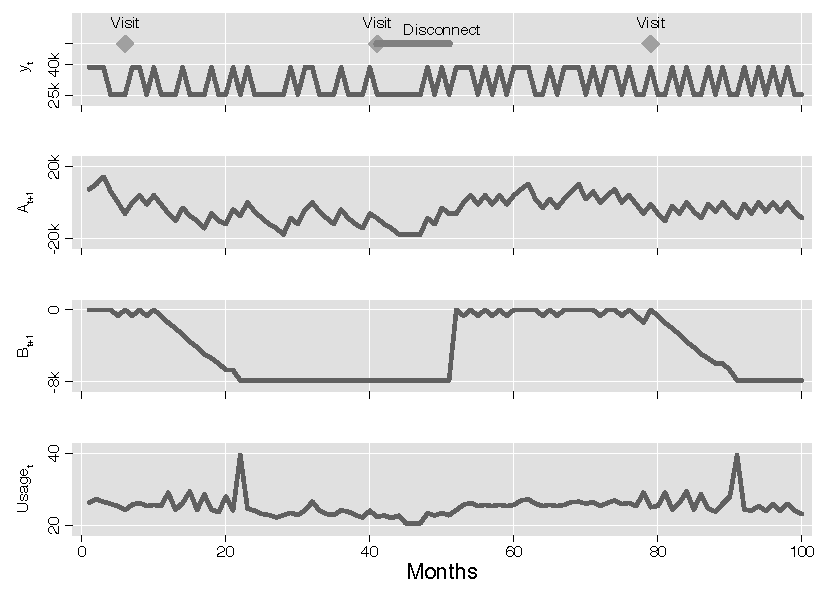
\includegraphics[scale=1.1]{tables/new_deaton_graph.pdf} \\
% {\scriptsize  
% Note: 100 months are chosen to center around the first disconnection event in the  2,000
month random sequence of income and delinquency visit states used in the estimation.  ``Visit'' indicates months with a delinquency visit with a diamond.  ``Disconnect'' indicates months disconnected with a thick line.  Cum. $\Delta y_t$ measures cumulative shocks to income in PhP, $A_{t+1}$ indicates the optimal position for standard assets in PhP, $B_{t+1}$ indicates the optimal amount of water borrowing in PhP, and $\text{Usage}_t$ indicates water consumption in m3.
% \par}
% \end{figure}


To build intuition, Figure~\ref{figure:deaton} provides 100 time periods of simulated data from the model.  These 100 time periods are chosen to center around the first disconnection occurrence in the  2,000
month random sequence of states used in the estimation.  The first panel in Figure~\ref{figure:deaton} indicates the cumulative, exogenous income shocks faced by the household.  This sample begins with a long period where negative income shocks occur more frequently than positive income shocks.  Positive shocks only begin to outweigh negative shocks at around 50 months.  Indicators for when the household receives delinquency visits as well as whether it chooses to remain disconnected are also nested in this first panel.  Over the course of 100 months, the household experiences three visits, the second of which leads the household to disconnect for around 12 months.  This disconnection corresponds to a period where the household has accumulated a long string of negative income shocks.

The second panel indicates the household's choice of asset position, $A_{t+1}$, in each month.  Asset position closely tracks income realizations as the household increasingly borrows (moving into very negative positions) following the long series of negative income shocks.  At around the time of disconnection, the household chooses to borrow the maximum allowed by the grid of assets chosen for the simulation.  Positive income shocks then allow the household to borrow less and begin saving at around 60 months.

The third panel indicates household borrowing through unpaid water bills, $B_{t+1}$.  In the beginning, the household increases its borrowing more slowly than with standard assets since each month's increase in borrowing is limited by the size of the household's current water bill.  Matching the downturn in income, the household continues borrowing before reaching the maximum borrowing allowed by the grid of assets chosen in this simulation.  With few positive income shocks, the household remains at this maximum borrowing level for at least 24 months.  When the second delinquency visit occurs at around 40 months, the household is still borrowing the maximum from unpaid water bills and therefore, instead of choosing to pay its full outstanding balance to stay connected, the household chooses to disconnect until it accumulates enough positive income shocks to pay its full water bill around month 55.  During the third delinquency visit, the household's outstanding balance happens to be relatively small so it is able to immediately pay in full to remain connected.

\todo[color=green]{Why lumpy/spikey? Why doesn't usage just go up smoothly?}The fourth panel indicates household water usage patterns over the same 100 months.  Usage begins to spike as the household increases its usage to fund borrowing through unpaid water bills.  The largest spikes in usage occur when the household moves to the maximum level of borrowing.  Because of the step-size chosen for the asset grid, moving to the largest borrowing level requires a jump in unpaid bills of around 1,000 PhP.  Since the average bill is around 600 PhP, the household needs to almost double its usage to fund this jump in borrowing from unpaid bills.  These spikes in usage measure the extent to which borrowing from unpaid water bills may distort consumption choices, adding an additional friction associated with borrowing from water bills.  After maximizing water borrowing at around 24 months, usage begins to stabilize at lower levels, mirroring the long string of negative income shocks faced by the household.  Usage recovers to a higher level after the second delinquency visit before spiking again as the household maximizes its water debt in the last several months.\todo[color=green]{If this is just a grid-size quirk, don't highlight it like its!  Borrowing limit is awkward}





\section{Counterfactual Policies}\label{section:counterfactuals}
% The institutional context in Manila provides a useful setting to quantify welfare effects because the

The estimated model allows for simulating the welfare effects of counterfactual billing policies.  The first counterfactual implements a prepaid metering system that requires households to pay upfront for their water consumption.  This system prevents households from timing their bill payments to smooth their consumption.  The second counterfactual halves the frequency of disconnection warnings.  This policy encourages households to accumulate large unpaid bills and smooth their consumption. 

These policies are paired with price adjustments that ensure that the utility's revenues always equal its costs.  This revenue-neutral approach reflects how governments in Manila and many other countries regulate utility prices (\cite{hoque2013state}).  Since utility profits are held constant, changes in household welfare summarize the total welfare effects of the counterfactual policies.  

The counterfactual policies account for changes in three types of operating costs: 
\begin{enumerate}
	\item \textit{Lending Costs}:  By tolerating unpaid bills, the utility extends credit to households each month at zero interest rate.  The opportunity cost of this credit is equal to the 0.47\% monthly interest rate that the utility pays on its loans to fund its own capital investments.\footnote{The 0.47\% monthly interest rate is equal to a 5.75\% annual interest rate.}  The utility also loses revenue from households that leave unpaid bills when they disconnect.  Therefore, expected lending opportunity costs per household can be expressed as $ - \chi B_T + \sum_{t=1}^{T}  - 0.0047 B_t $ where $B_t$ ($<0$) equals unpaid bills each month and $\chi$ is the share of households that leave unpaid bills upon disconnection.

	\item \textit{Warning Costs}:  The utility incurs costs visiting and warning each delinquent household about their unpaid bills.  The cost of administering each warning is  assumed to equal the reconnection fee of 200 PhP.\footnote{Conversations with the utility suggest that travel costs make up the majority of the costs for any service performed on a water meter.}  Warning costs per household can be expressed as  $\sum_{t=1}^{T} 200 \lambda \mathbbm{1}\{B_t < 0 \}  $ where $ \mathbbm{1}\{B_t < 0 \}$ indicates months where households are delinquent and $\lambda$ indicates the share of months where the utility conducts warnings.

	\item \textit{Pumping Costs}: The utility estimates that the marginal cost of supplying a cubic meter of water is equal to 5 PhP.  The total marginal costs per household can be expressed as $\sum_{t=1}^{T} 5 w_t  $ where $w_t$ reflects monthly water consumption.
\end{enumerate}
Under Manila's price regulations, total revenue net of operating costs equal the fixed costs of building and maintaining the pipe network.  Therefore, fixed costs are measured as observed revenue net of observed operating costs according to the following equation
\begin{align}
\label{utilitybc}
\sum_{t=1}^{T} FC = \underbrace{\sum_{t=1}^{T} (p_1+p_2 w_t)w_t}_{\text{Revenue}}  - \Big[ \underbrace{-\chi B_T +  \sum_{t=1}^{T} 5 w_t + 200 \lambda \mathbbm{1}\{B_t < 0 \} - 0.0047 B_t}_{\text{Operating Costs}} \Big]
\end{align}
where $FC$ equals fixed costs in monthly terms.  Fixed costs are assumed to remain constant in counterfactual simulations.  As each counterfactual policy changes household consumption and billing patterns, the simulation adjusts the marginal price per cubic meter, $p_1$, to satisfy  equation (\ref{utilitybc}).






\begin{table}[H]
\centering
\caption{Counterfactual Policies}\label{table:counter}
\resizebox{\columnwidth}{!}{%
\begin{threeparttable}
\begin{tabular}{l*{1}{EEE}}
\toprule
 & (1)     & (2)          & (3)   \\
 & Current & Prepaid Metering & 50\% Less Enforcement   \\
\midrule
Compensating Variation &   & 109
  & -117
  \\[.2em]
Average Consumption			 &   631
 & 545
    &  613
 \\[.2em]
Average Outstanding Balance & 1231
 & 0
    &  3185
  \\[.2em]
Price per m3  &  17.6
 & 14.8
    &  16.7
  \\[.2em]
Share of Months with Delinquency Warnings & 0.22
& 0.00
  & 0.11
  \\
\bottomrule
\end{tabular}
\begin{tablenotes}
\item \footnotesize 
Compensating variation measures the change in monthly income needed to make households indifferent between the current scenario and the counterfactual scenario.  Average consumption and outstanding balance are measured monthly in PhP.  Price per m3 reflects the constant marginal price per m3, $p_1$, so that total price equals $p_1+p_2 w_t$ where $w_t$ is monthly consumption in m3. 
\end{tablenotes}
\end{threeparttable}
}
\end{table}




% Counterfactual simulations equate revenues with costs by either charging a fixed monthly fee or providing a fixed monthly rebate to households.\footnote{In practice, the utility charges households a small monthly fixed fee to cover some meter and pipe maintenance costs even households are temporarily disconnected.}  This approach preserves the utility's marginal prices because they may reflect the government's distributional preferences or attempts to mitigate environmental externalities.

Prepaid meters may generate cost savings by eliminating the need to enforce payments and preventing households from leaving unpaid balances upon disconnection.  Any cost savings are passed onto households through lower prices.  At the same time, prepaid meters may reduce household welfare by preventing households from timing their bill payments to smooth their consumption.



 % While this policy may generate cost savings , the utility may also lose revenue when households leave large unpaid bills upon disconnection.  

I then simulate the effects of introducing prepaid metering technologies and adjusting water prices to similarly account for their costs.  By requiring households to pay upfront for their water usage, these meters provide an alternative strategy for eliminating unpaid water bills.  These technologies have become increasingly popular for both electricity and water utilities throughout the developing world.\footnote{See \cite{jack2016charging} and \cite{northeast2014} for electricity utilities and \cite{heymans2014limits} for water utilities.}  These technologies may be especially useful in contexts where other factors drive delinquency instead of consumption smoothing.   For example, \cite{szabo2015reducing} suggest that low levels of trust in local government and perceptions of fairness may drive some nonpayment behavior.  While these factors are not explicitly modeled in this context, this exercise may still provide a useful lower bound for evaluating the welfare effects of prepaid metering programs.


In the counterfactual, cost savings reduce the amount of revenue needed to be raised to stay revenue neutral.  At the same time, eliminating borrowing in the counterfactual lowers water consumption, which reduces revenue since prices are well above marginal costs.  Table~\ref{table:counter} finds that these two effects almost exactly offset each other, producing almost identical prices in the current setting in Column (1) and in the counterfactual without water borrowing in Column (3).  Removing water borrowing while keeping similar prices results in a drop in average usage between Columns (1) and (3) that is nearly identical to the drop in usage between Columns (1) and (2).

According to the first row of Table~\ref{table:counter}, households would require a compensating monthly payment of at least 89.4
PhP in order to move from the current setting in  Column (1) to a revenue-neutral counterfactual without borrowing in Column (3).  Although prices remain almost identical in Column (3), revenue neutrality ensures that households no longer receive a monthly disconnection rebate of 10.2PhP, which almost exactly accounts for the difference in compensating variation between columns (2) and (3).  




Prepaid meters introduce an additional cost for the utility in terms of purchasing and installing this new technology.  \cite{heymans2014limits} surveyed eight large water providers that implemented prepaid meters in developing countries and found that each prepaid meter costs about four times as much as a standard meter and requires replacement every 7 years.  In the context of Manila, each standard meter costs around 1,500 PhP and is replaced around every 6 years and 3 months, bringing the monthly cost to 20 PhP/month.\footnote{The utility provided additional documentation of their costs and frequency of meter replacement for residential households.}  Assuming that a prepaid meter costs 4 times as much as a standard meter with a replacement rate of 7 years, the estimated monthly cost of a prepaid meter would be 71 PhP/month.  Therefore, prepaid meters imply an additional cost of 51 PhP/month per household.\footnote{\cite{heymans2014limits} also report that the fixed administrative costs of installing and monitoring new meters account for less than 4\% of the total costs of switching to prepaid meters while the bulk of the expenses come from purchasing new meters.  By focusing on meter replacement, this exercise is likely to capture the majority of switching costs associated with prepaid metering.}  

Column (4) of Table~\ref{table:counter} includes the results of the prepaid metering counterfactual.  To cover the much higher costs of prepaid meters, the price intercept, $p_1$, increases by around 18.3
\unskip\% as indicated by the fourth row.  Households also no longer receive a disconnection rebate of 10.2PhP per month.  With higher prices and without water credit, households lower their consumption by 12.7
\unskip\% under prepaid metering compared to the current setting in Column (1).  In order to be indifferent between the current setting and a counterfactual with prepaid metering, households would need to receive 245.5
PhP/month in compensation.  Taken together, these results provide suggestive evidence that prepaid metering would reduce welfare substantially in this context.







% added footnote which might deal with it, but think harder on it later --- deal with this? - in practice, the utility charges a fixed price... not model or introduce in the model earlier???



- 







To measure how much households value credit from unpaid water bills, I examine how household welfare changes in a counterfactual setting where households are unable to borrow from their water bills.  Table~\ref{table:counter} includes outcomes for the current setting in Manila in Column (1) and for a counterfactual setting without water borrowing in Column (2), which is captured by raising the interest rate on unpaid water bills to 100\% and holding all else equal.  The first row calculates compensating variation equal to 50.3
PhP (or 1.5
USD) per household-month associated with losing access to water credit.  This estimate suggests that households are indifferent between their current situation and a counterfactual with 50.3
PhP per month in additional income and without access to water credit.  Given an average water bill of 691.6PhP/month, this estimate would translate into households paying around 8
\unskip\% smaller bills each month.  

Eliminating credit access also decreases mean usage by 6.0
\unskip\% as shown by columns (1) and (2) in the second row of Table~\ref{table:counter}.  Eliminating credit access lowers the extent to which households can smooth their consumption over time while also removing the incentive for households to overconsume water in order to finance water borrowing.  Given that households spend around 2.2\unskip\% of their income on water, this estimate is roughly proportional to similar evidence from South Africa where restricting credit access with prepaid electricity meters produced a 13\% reduction in usage and where households spend around 8-10\% of their income on electricity (\cite{jack2016charging}).\footnote{\cite{jack2016charging} also propose other mechanisms that may account for reductions in usage such as transaction costs and intra-household bargaining constraints.}





%\subsection{Prepaid Metering}

This setting also provides a useful opportunity to simulate the social welfare impacts of popular policies to reduce delinquency.  I consider a policy that (1) eliminates borrowing by raising the interest rate on unpaid bills to 100\% and (2) adjusts prices to ensure that the utility remains revenue-neutral.  The regulatory structure in Manila as well as many other developing cities ensures that prices for water are regulated to exactly cover all production costs .

Eliminating borrowing affects the costs of the utility in four main ways

To determine price increases necessary to cover these costs, the following expression first calculates the revenue raised through prices,  $p_1$ and $p_2$, per household-month given income, $Y$, net of marginal cost, $MC$
\begin{align*}
REV \big(p_1,r_b,Y \big) &= \Big ( \,  p_1 - MC +  p_2 \, w^{*}(p_1,p_2,r_b,Y)  \,  \Big ) \, \, w^{*}(p_1,p_2,r_b,Y)
\end{align*}
%With prepaid meters, the  utility would also no longer need to conduct delinquency visits.  

%Appendix~\ref{appendix:visitcosts} provides evidence that these cost savings are likely to be negligible.

I then solve for the new price intercept, $p^{\prime}_1$, such that the current revenue is equal to revenue under a counterfactual where the borrowing rate is equal to 100\% and the utility enjoys cost savings.   This exercise assumes that the government regulator is able to perfectly forecast water demand among all households.  Adjusting only the price intercept, $p^{\prime}_1$, instead of both price terms provides a way of preserving the slope of the tariff structure, which likely reflects equity concerns among policymakers in Manila.  

$p^{\prime}_1$ is chosen to solve the following expression
\begin{align*}
\sum_t REV_t \big(p_1,0,Y_t \big) =& \sum_t REV_t \big(p^{\prime}_1,1, Y_t - \text{Disc. Rebate} \big) \\
& - (\text{Opp. Cost of Lending + Visit Cost + Disc. Rebate})
\end{align*}


%%% also include counterfactual where we increase the interest rate and see substitution? may have to rewrite some of the identification section....

\section{Conclusion}\label{section:conclusion}

Prepaid meters for electricity already compose over 27.5\% of residential meters in Sub-Saharan Africa and are predicted to grow to 52.8\% by 2024 (\cite{northeast2014}).  Similarly, by planning to install over 300,000 prepaid meters, the Botswana Water Utilities Corporation provides an example of the growing use of this technology in the water sector (\cite{heymans2014limits}).  Policy proposals for prepaid meters often emphasize how this technology ensures cost-recovery for utility providers.  At the same time, households stress how ``water is a need, but money is not always available'' and  how ``postpaid gives you more time to find the money'' in qualitative evidence documented by \cite{heymans2014limits}.  These anecdotes suggest a potentially important role for billing flexibility in allowing households to smooth consumption.  

This paper builds a dynamic model of household consumption smoothing to measure the extent to which households value billing flexibility.  Estimates imply that households' valuation of flexibility is on the order of 8
\unskip\% of their monthly water bills.  Counterfactual exercises further find that policies to eliminate nonpayment --- raising interest rates on unpaid bills and prepaid metering --- do not produce enough cost savings to justify their negative impacts on household consumption smoothing.\todo[color=red]{i'm still not sure i get this... what are the cost savings?}  On net, these policies are predicted to reduce social welfare by between 2.0
and 5.0
USD per household-month.  \todo[color=red]{i would add more oomph to this. i think this is really interesting but the punchline needs to be bigger!}

In focusing on the role of consumption smoothing, this approach abstracts away from other channels by which nonpayment may affect welfare.  First, high rates of nonpayment may weaken incentives for utilities to invest in and extend access to high quality infrastructure.  While regulators in Manila successfully ensure universal access and service quality, \cite{mcrae2015infrastructure} documents how electricity providers in Colombia often shirk on infrastructure investments in areas where they face high levels of nonpayment, which are also often underprivileged areas.  Second, policing nonpayment through unexpected disconnections may also have unintended health consequences (\cite{franklin2017}).  The US Department of \cite{liheap} lists a series of state-level policies restricting disconnections, especially in months with extreme temperatures, for public health reasons.  Finally, nonpayment may provide a way for households to voice their dissatisfaction with a utility as well as local government.  \cite{szabo2015reducing} find evidence that reaching out to consumers on behalf of a water utility increased payments from households motivated by a sense of reciprocity.  

%Third, \cite{jack2015pay} also argue that prepaid meters may help savings constrained consumers by allowing low-income households to pay in small increments each month.

% The counterfactual exercises constructs a framework for incorporating households' demand for consumption smoothing into evaluations of prepaid meters and other policies to reduce nonpayment.  

% By focusing on consumption smoothing, this paper abstracts away from several other consequences of utility billing policy.  First, many governments require utilities to tolerate nonpayment due to health concerns.  For example, the NAACP cites stuff ....  cite some more of Jack!! what mechanisms? savings constraints?  intrahousehold bargaining; go look up her new paper!!!!



% https://liheapch.acf.hhs.gov/Disconnect/disconnect.htm

%% compared to prepaid electricity
% • Prepaid water is often seen as controversial. Payment for the supply of electricity is accepted more widely than
% payment for water, and access to electricity is not regarded a basic human right. T
% • The electricity sector is much less fragmented than the water sector, and has far greater clout to direct what
% manufacturers supply. 
% • Prepaid water meters face physical stresses that do not apply to electricity. There are more moving parts,
% most subjected to fluctuating pressures and flows, and wear, fatigue, and abrasion increase the likelihood of
% malfunction. 


% When discussing costs with service providers, the review
% team was told on several occasions that “prepaid meters cost
% about four times more than a conventional meter.” This is
% based on the typical cost of a prepaid metering device for an
% individual domestic connection, about US$210, compared
% to typical conventional mechanical meter, about US$50.   96.2\% of costs for large systems.  average of 7 year life span (assume the same for both)


% \cite{northeast2014} predict rapid increases in prepaid electricity meters throughout Sub-Saharan Africa.  

% \cite{heymans2014limits}
%  prepayment water systems are in use in more than
% 20 African countries, and in locations such as Turkey, parts
% of the Balkans and Azerbaijan, and Colombia. Their scale
% of use is ramping up rapidly. The Botswana Water Utilities
% Corporation, for example, is reported to be planning to install
% 300,000 prepaid water meters in the near future, beyond
% the existing small-scale installations. 

%  don't like : “Postpaid gives you more time to find the money.”  “Water is a need, but money is not always available.”






\section{Appendix}



\subsection{Sample Construction}\label{appendix:sampleconstruction}

Merging the full sample from the connection survey to the billing data yields an initial population of 798,223connection-months as described in Table~\ref{table:sampleconstruction}.  Non-residential accounts are first removed to ensure that results apply to household-level decisions.  Due to some data inconsistencies, payment records are missing for some connections, which are excluded.  Due to leaks, meter replacements, and meter reading errors, connections occasionally experience extremely high meter readings and bills.  Consumption records above 200 m3 as well as bills and payments above 80,000 are censored to address these issues.  Large negative payments and outstanding balances (due to reimbursements of billing errors) are also excluded due to likely measurement error.  Remaining negative payments and balances likely represent refunds to households (possibly due to system errors), which are included to accurately reflect each household's asset position.  Households that connect during the sample or have large stretches of missing records are excluded by including only connections with over 30 months of data.  Keeping only connections serving single households brings the final sample size to 2,030,876household-months.


\begin{table}[H]
\centering
\caption{Sample Construction}\label{table:sampleconstruction}
\vspace{-2mm}
\resizebox{\columnwidth}{!}{%
\begin{tabular}{l*{1}{cc}}
\toprule
 & Observations & Observations Removed  \\
\midrule
Initial sample   &         798,223  &     \\
Keep residential connections (excluding commercial)   &            &    102,415  \\
Keep connections with payment records &  &   40,708   \\
Keep months with usage under 200 m3    &            &  73,219     \\
Keep bills $>$ -5,000 PhP and $<$ 80,000 PhP  &  & 116  \\
Keep unpaid bills $>$ -5,000 PhP and $<$ 80,000 PhP &             &     844  \\
Keep payments $>$ -80,000 PhP and $<$ 80,000 PhP    &            &    1   \\
Keep connections with over 30 months of records   &            &   218    \\
% Keep connections serving a single household   &            &   721,146    \\
%Drop connections that are disconnected for final yr.  &            &   92,459    \\
Final sample & 2,030,876 & \\
\bottomrule
\end{tabular}
}
\end{table}


\subsection{Bill Payments and Delinquency Warnings}\label{appendix:paywarning}

The following equation estimates the effect of delinquency warnings on bill payments
\begin{align*}
Pay_{it} = \alpha &+ \beta  \{ \text{own warning} \}_{it} + \\
 &\sum_{k=1}^{3} \gamma_k \{ \text{warning for k-th nearest HH in same neighborhood} \}_{it} +  \\
 &\sum_{j=1}^{3} \theta_j \{ \text{warning for j-th nearest HH in different neighborhood} \}_{it} + \eta_i + \zeta_t + \epsilon_{it}
\end{align*}
where $i$ indexes households and $t$ indexes months.  $Pay$ indicates bill payments in the same month.  Indicators variables signal months where households receive warnings and where their three immediate neighbors receive warnings.  Immediate neighbors are considered separately based on whether neighbors reside in the same or different neighborhoods.  The specification also includes household fixed effects ($\eta_i$) and calendar month fixed effects ($\zeta_t$).  Information on the exact location of each household is available for over half of the sample, which is used to measure distances between households.

Table~\ref{table:paywarning} includes the results of this exercise.  Receiving a delinquency warning is correlated with large, immediate increases in bill payments around the size of the average bill payment in the sample.  Conditional on receiving a warning, households that have immediate neighbors who receive warnings in the same neighborhood also increase their bill payments although the magnitudes are much smaller than the own warning effect.  Warnings for the 3rd nearest household have a slightly smaller effect than warnings for the nearest household although warnings for all households are positive and significant.  Households do not appear to change their payment behavior when nearby households in different neighborhoods receive warnings, which suggests that the utility follows a neighborhood sweeping strategy.

\begin{table}[!ht]
\small
\centering
\begin{threeparttable}
\caption{Bill Payments and Delinquency Warnings}\label{table:paywarning}
\vspace{-2mm}
% \resizebox{.8\linewidth}{!}{
\begin{tabular}{lc}
\toprule
 % & \small (1)  \\
 & \small Bill Payment (PhP) \\[.5em]
 \toprule
Own Warning         &      587.51\textsuperscript{a}\\
                    &     (19.73)                   \\[0.5em]
Warning in Same Neighborhood for: \\[.5em] \hspace{.5em}1st Nearest Household&       42.36\textsuperscript{a}\\
                    &     (11.67)                   \\[0.1em]
\hspace{.5em}2nd Nearest Household&       46.63\textsuperscript{a}\\
                    &     (11.06)                   \\[0.1em]
\hspace{.5em}3rd Nearest Household&       33.56\textsuperscript{a}\\
                    &     (11.67)                   \\[0.1em]
Warning in Different Neighborhood for:  \\[.5em] \hspace{.5em}1st Nearest Household&       10.97                   \\
                    &     (33.01)                   \\[0.1em]
\hspace{.5em}2nd Nearest Household&       -6.11                   \\
                    &     (28.85)                   \\[0.1em]
\hspace{.5em}3rd Nearest Household&        7.58                   \\
                    &     (25.21)                   \\[0.1em]
Mean                &      629.40                   \\
$\text{R}^{2}$      &       0.286                   \\
N                   &   1,148,439                   \\

\bottomrule
\end{tabular}
\begin{tablenotes}
\footnotesize
\item Household and calendar-month fixed effects are included. Standard errors are clustered at the household level.  \textsuperscript{c} p$<$0.10,\textsuperscript{b} p$<$0.05,\textsuperscript{a} p$<$0.01 
\end{tablenotes}
\end{threeparttable}
\end{table}


\subsection{Average Unpaid Bills Before Permanent Disconnection}\label{section:billtodc}


\begin{figure}
\caption{Average Unpaid Bills in 36 Months Before Permanent Disconnection}\label{figure:billtodc}
\begin{center}
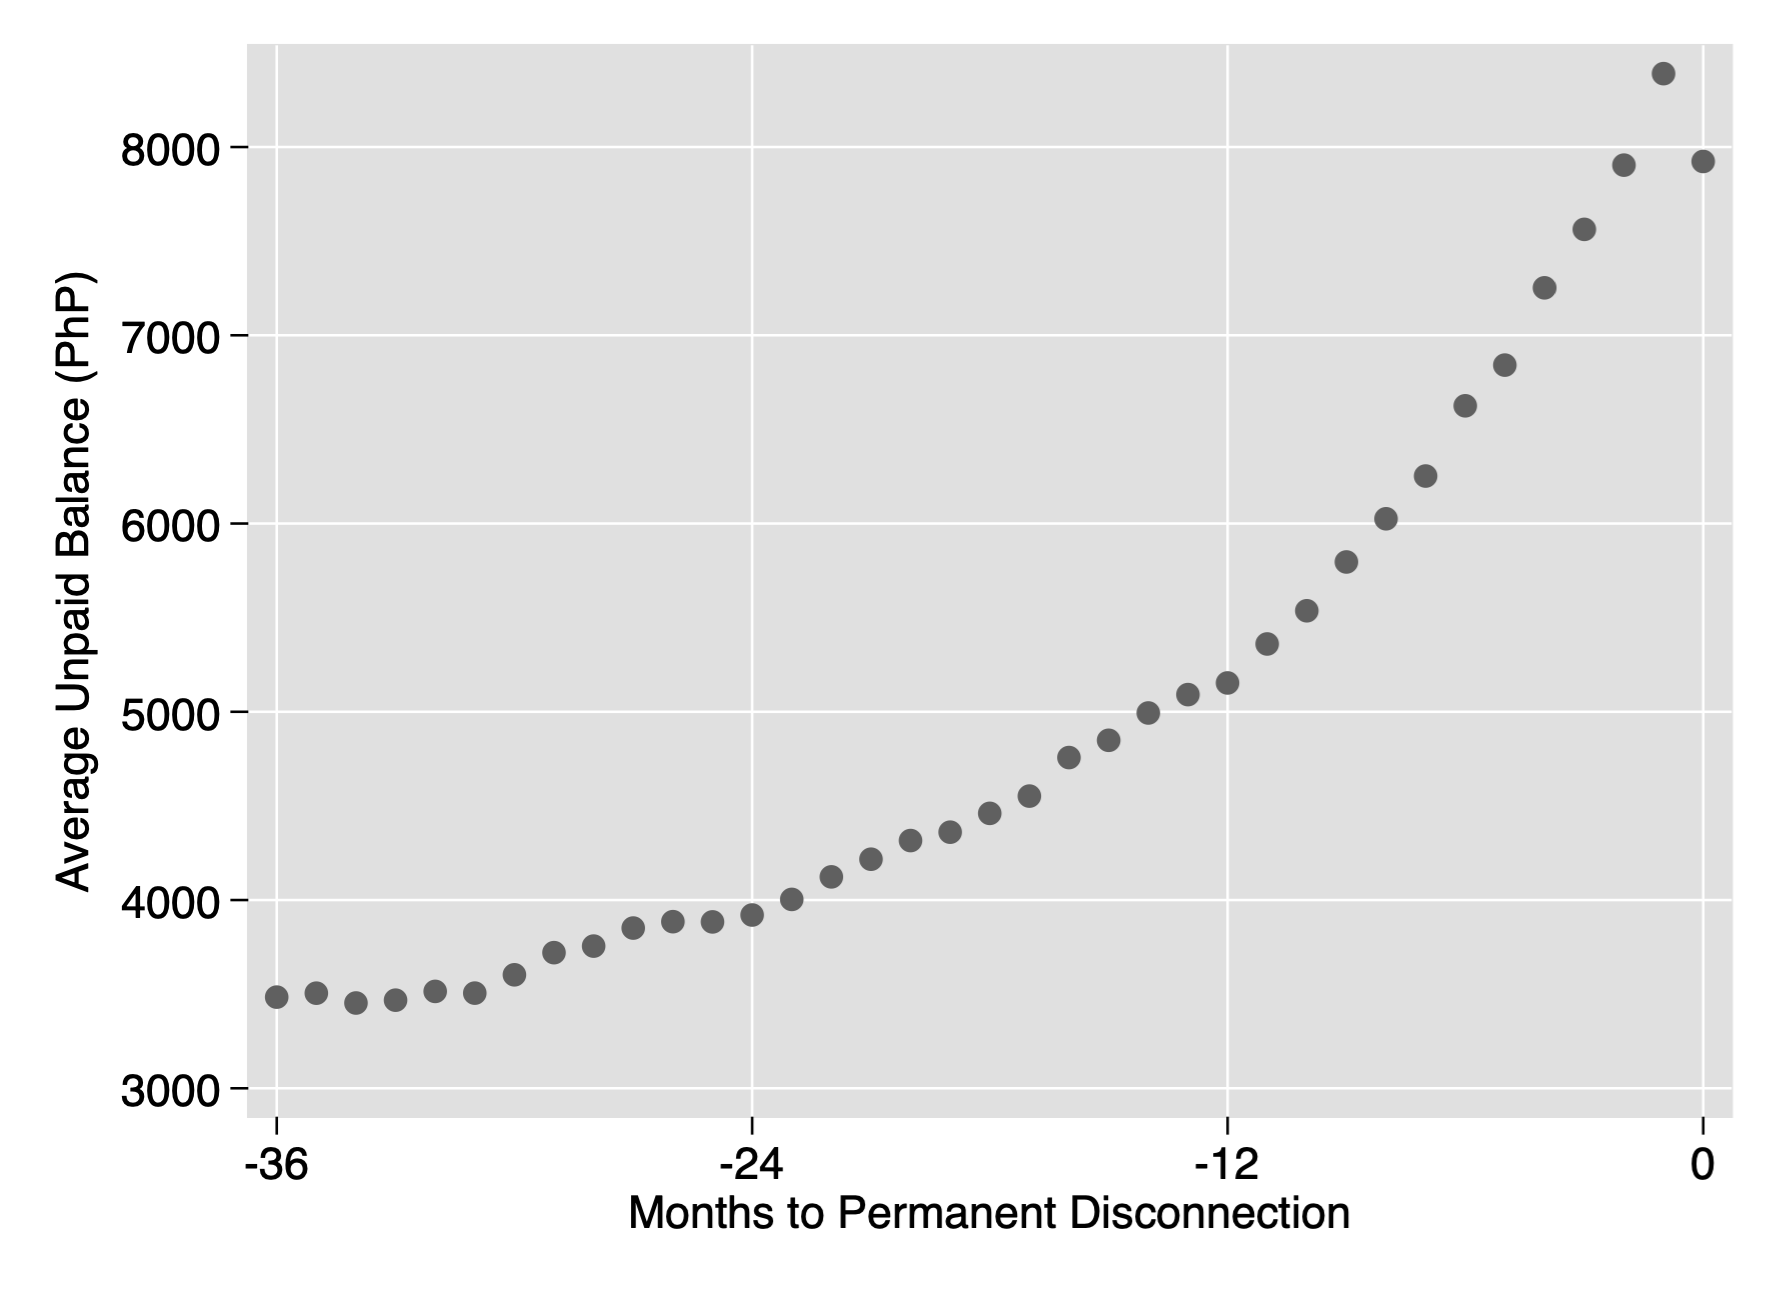
\includegraphics[scale=.4]{tables/pay_to_dc_graph.png}
\end{center}
\end{figure}


% \subsection{Shape of the Utility Function}\label{appendix:utilityshape}

% Log-utility is a special case of Constant Relative Risk Aversion (CRRA) utility given by $u(c) = \frac{c^{1-\rho}}{1-\rho}$ when $\rho=1$.  CRRA is one of the most popular functions for risk aversion in the economics literature (\cite{wakker2008explaining}).  The literature provides a range of estimates for $\rho$ which are above, below, and around one.  \cite{barseghyan2013nature} use insurance choices in the US to estimate a $\rho$ between 0.21 and 0.37.  \cite{beetsma2001measuring} use a natural experiment from a Dutch game show to estimate $\rho$ ranging from 0.42 to 6.99.  \cite{carvalho2016effect} leverage an experimental setting in Nepal to estimate $\rho$ equal to 0.63.  Given these estimates, assuming $\rho$ equal to one implies a moderate curvature of the utility function and is relatively close to a comparable estimate from a development economics setting.  

% \subsection{Indirect Utility Function}\label{appendix:indirectutil}

% \begin{align}\label{eq:vstar}
% \begin{split}
% v^{*} &= 
% \begin{cases}
% \alpha \,\ln(\frac{p_{1}-\sqrt{{p_{1}}^2-8\,L\,\alpha \,p_{2}+8\,Y\,\alpha \,p_{2}+4\,L\,\alpha ^2\,p_{2}-4\,Y\,\alpha ^2\,p_{2}}}{2\,p_{2}\,(\alpha -2)})- \\ \ln(\frac{(\alpha -1)\,(8\,L-8\,Y-4\,L\,\alpha +4\,Y\,\alpha )}{2\,{(\alpha -2)}^2}+ \\
% \frac{(p_{1}\,\sqrt{{p_{1}}^2-8\,L\,\alpha \,p_{2}+8\,Y\,\alpha \,p_{2}+4\,L\,\alpha ^2\,p_{2}-4\,Y\,\alpha ^2\,p_{2}}-{p_{1}}^2)\,(\alpha -1)}{2\,p_{2}\,{(\alpha -2)}^2})\,(\alpha -1)\\
%  &\text{ if } L \geq \widehat{L} \\
%                                                                                                                                                                                                                                                                                                                                                                                              \alpha \,\ln\left(-\frac{p_{1}-\sqrt{{p_{1}}^2-4\,L\,p_{2}}}{2\,p_{2}}\right)-\ln\left(Y\right)\,\left(\alpha -1\right)
 &\text{ if } L < \widehat{L}
% \end{cases} \\
% &\widehat{L} =                                                                                                                                                                                                                                                                                                                                 \frac{Y}{2\,\left(\alpha -1\right)}+\frac{\frac{Y\,p_{2}}{2}+\frac{{p_{1}}^2}{8}-\frac{p_{1}\,\sqrt{{p_{1}}^2-\alpha \,{p_{1}}^2+8\,Y\,\alpha \,p_{2}}}{8\,\sqrt{1-\alpha }}}{p_{2}}

% \end{split}
% \end{align}



\subsection{Tariff Structure and Approximation}\label{appendix:tariff}

% \begin{figure}
% \caption{Example Residential Tariff Presented to Consumers}\label{figure:tarifftrue}
% \begin{center}
% 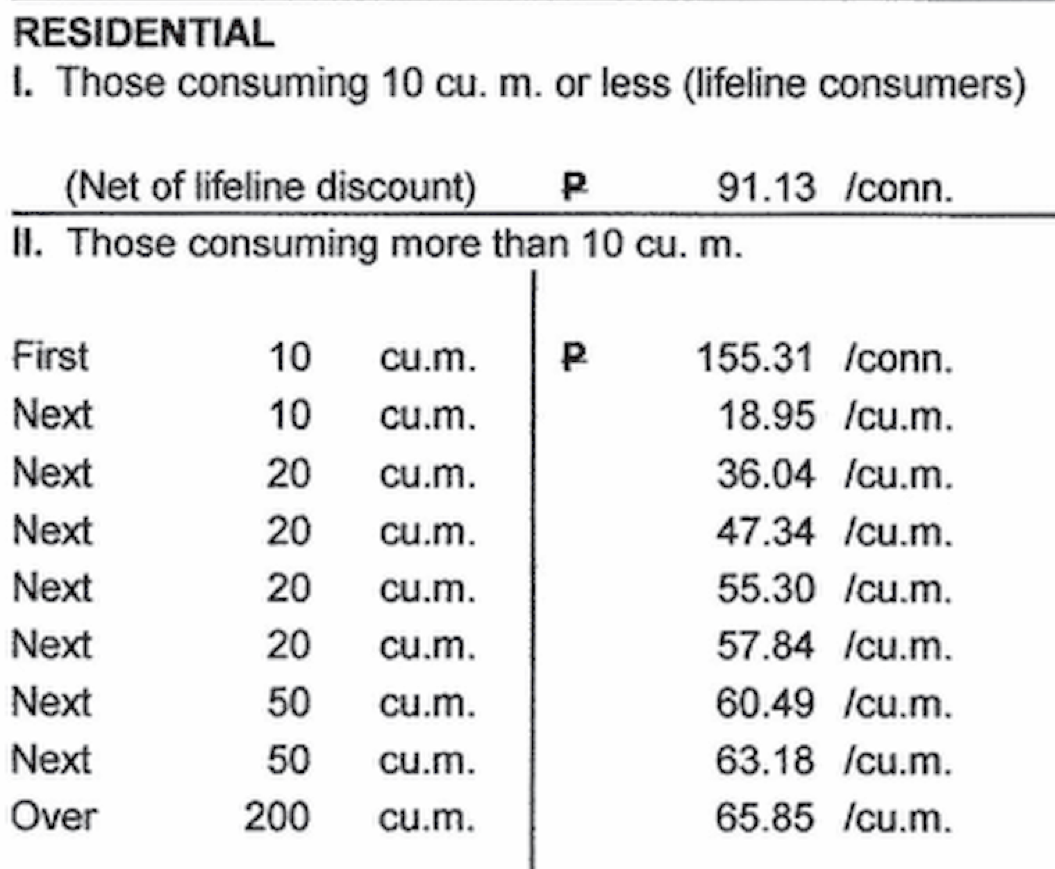
\includegraphics[scale=.8]{tables/tariff_pic_png.png} \\
% \footnotesize{``conn.'' refers to connection, ``cu.m.'' refers to cubic meters of usage \\ per month, and \textbf{P} refers to Philippine Pesos.  Includes Tariff as of February, 2019.}
% \end{center}
% \end{figure}


\begin{table}[H]
\centering
\caption{Example Residential Tariff As Presented to Consumers}\label{table:tarifftrue}
\vspace{-2mm}
\begin{tabular}{l*{1}{r}}
\toprule
Usage (m3) & Price (PhP) \\
\midrule
Under   10    &   104.12/conn. \\
Over    10    &   180.35/conn. \\
Next    10    &   19.20/cu.m. \\
Next    20    &   25.32/cu.m. \\
Next    20    &   33.21/cu.m. \\
Next    20    &   40.73/cu.m. \\
Next    20    &   45.92/cu.m. \\
Next    50    &   48.86/cu.m. \\
Next    50    &   55.31/cu.m. \\
Over   200    &   57.60/cu.m. \\
\bottomrule
\multicolumn{2}{l}{\scriptsize Mean tariff 2010-2015 with value added tax. }\\[-.5em]
\multicolumn{2}{l}{\scriptsize ``conn.'' refers to connection. }\\[-.5em]
\multicolumn{2}{l}{\scriptsize ``cu.m.'' refers to m3/month.  50 PhP$\sim$1 USD }
\end{tabular}
\end{table}

Table~\ref{table:tarifftrue} provides the monthly tariff structure as it is presented to consumers.  Consumers face a fixed price as well as marginal prices for any usage above 10 m3.  The regulator gradually adjusts prices at roughly yearly intervals in order to ensure that the utility is able to exactly cover its costs.  The marginal price is highly non-linear, accelerating quickly at low usage levels before slowly increasing at high usage levels.  To achieve a tractable approximation of this price schedule, Table~\ref{table:tcd_predict} fits a simple regression model predicting average price as a function of an intercept, $p_1$, and monthly usage levels, $p_2$.  This model predicts that a increase in monthly usage of 10 m3 results in an increase in average price of 2.2 PhP/m3.  

\begin{table}[H]
\small
\centering
\caption{Average Price and Monthly Usage}\label{table:tcd_predict}
\vspace{-2mm}
\begin{tabular}{lc}
\toprule
& \small Avg. Price: $\frac{\text{Bill (PhP)}}{\text{Usage (m3)}}$    \\
\midrule 
Usage (m3)          &        0.29\textsuperscript{a}\\
                    &      (0.00)                   \\[0.5em]
Intercept           &       17.53\textsuperscript{a}\\
                    &      (0.05)                   \\[0.5em]
Household-Months    &   1,946,309                   \\

\bottomrule
\multicolumn{2}{l}{\scriptsize \textsuperscript{c} p$<$0.10,\textsuperscript{b} p$<$0.05,\textsuperscript{a} p$<$0.01 }
\end{tabular}
\end{table}




\subsection{Alternative Income Test}\label{appendix:alternativeincome}

The following equation empirically tests whether income is more correlated with bill payments than with consumption
\begin{align*}
\Delta Y_{bq} = \beta\, \Delta \textsc{Income}_{bq} \,+\, \gamma_q \,+\varepsilon_{bq}
\end{align*}
where $\textsc{Income}_{bq}$ is proxied by the quarterly change in average labor earnings from Quarterly Labor Force Surveys where $q$ indexes 28 quarters from 2009 to 2015.  Average earnings are computed for 80 unique bins, $b$, defined by combinations of 4 sub-municipalities, age in 5 year intervals, and whether college educated in order to merge individuals from the Labor Force Survey to individuals water connection owners from the water connection survey.  $\Delta Y_{bq}$ is the quarterly change in either average water consumption (measured by the water bill in PhP) or average water bill payments (in PhP) by bin-quarter.  Standard errors are clustered at the bin-level.

\begin{table}[!ht]
\small
\centering
\begin{threeparttable}
\caption{Correlations of Income with Consumption and Payment Patterns}\label{table:lfsanalysis}
\vspace{-2mm}
% \resizebox{.8\linewidth}{!}{
\begin{tabular}{lcc}
\toprule
 & \small (1) & \small (2)  \\
 & \small $\Delta$ Consumption & \small $\Delta$ Payment \\[.5em]
 \toprule
$\Delta$ Employed   &     -0.0005                   &      0.0074\textsuperscript{b}&     -0.0076\textsuperscript{c}\\
                    &    (0.0071)                   &    (0.0034)                   &    (0.0044)                   \\[0.1em]
$\Delta$ Hours worked&     -0.0012                   &      0.0018                   &     -0.0017                   \\
                    &    (0.0028)                   &    (0.0016)                   &    (0.0025)                   \\[0.1em]
N                   &     512,978                   &     554,228                   &     554,228                   \\

\bottomrule
\end{tabular}
\begin{tablenotes}
\footnotesize
\item All units are in PhP.  Quarterly fixed effects are included.  Standard errors are clustered by age-group, sub-municipality, and whether college educated (80 units).  \textsuperscript{c} p$<$0.10,\textsuperscript{b} p$<$0.05,\textsuperscript{a} p$<$0.01 
\end{tablenotes}
\end{threeparttable}
\end{table}

Column (1) of Table~\ref{table:lfsanalysis} finds a positive but statistically insignificant correlation between income and consumption.  Due to measurement error in income, the small point estimate of 0.0007 likely underestimates this correlation.  Measurement error in income is likely to be substantial both because only around 55 incomes are observed per quarter-bin in the Labor Force Survey and because bins are constructed from coarse demographic categories that may only loosely reflect household incomes.  Despite this potential measurement error, Column (2) finds a statistically significant correlation between bill payments and income that is six times larger than the correlation between income and consumption.  These results provide suggestive evidence of consumption smoothing where households flexibly adjust their payment patterns in response to income shocks without changing their water consumption.  



\subsection{Usage Before Permanent Disconnection}\label{appendix:permanentdc}

%%% DISCUSS AVERAGE LENGTH OF ACCOUNTS IN THE SAMPLE!!!

% Figure~\ref{figure:dc_permanent} plots average usage across households according to the number of months before these households permanently disconnect. Average consumption increases in the months leading up to permanent disconnection.  This increase is likely due to some households using water as if they faced a zero marginal price since they know that they will never pay their bills.  With an average bill of 691.6PhP/month, leaving an outstanding balance of 7,119PhP at permanent disconnection is equal to enjoying an average of around 18 months of free water consumption.

\begin{figure}[H]
\centering
\caption{Average Usage in Months Before Permanent Disconnection}\label{figure:dc_permanent}
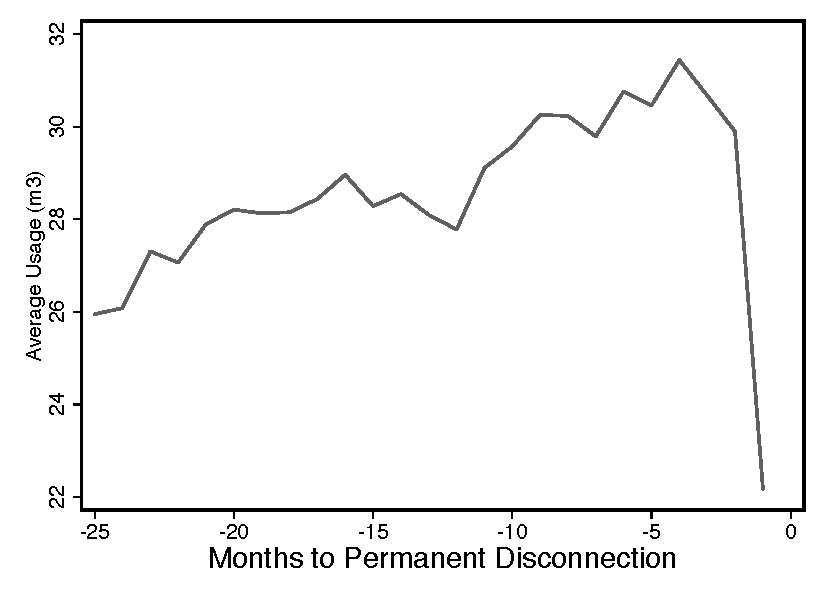
\includegraphics[scale=.7]{tables/line_disc_graph.pdf} \\
{ \footnotesize Permanent disconnection is defined as households disconnecting and remaining disconnected for the at least the last two years of the sample.  Negative months indicate months leading up to permanent disconnection.  Months with zero usage are dropped because households may leave months with zero consumption before the company disconnects them. }
\end{figure}


\subsection{Calibrated and Assumed Parameters}\label{section:calibratedparam}

\begin{table}[H]
\centering
\caption{Calibrated and Assumed Parameters}\label{table:calibratedparam}
\vspace{-2mm}
\resizebox{\columnwidth}{!}{%
\begin{tabular}{l*{1}{ccl}}
\toprule
%Parameter  &   &  Value & Source \\
%\midrule
% Savings Interest Rate & $r_l$ & 9.5\unskip\%  & {\footnotesize Philippines data from World Bank Databank (2010-2015) } \\
Mean Income (PhP) & $\bar{y}$ & 31,910 & {\footnotesize Pasay City Household Panel Survey} \\
Income Coefficient of Variation & $\theta$ & 0.52 & {\footnotesize  Pasay City Household Panel Survey} \\
Interest Rate on Standard Borrowing & $r$ & 9.5\unskip\% & {\footnotesize  Consumer Finance Survey for Manila} \\
Tariff    & $(p_1 + p_2 w)$ & $(20.226 + 0.3w)$ & {\footnotesize Estimated price by water usage  (See Appendix~\ref{appendix:tariff} for details) } \\
Discount Rate & $\delta$ & 0.5\% & {\footnotesize In range of structural estimates from $\text{literature}^{\dagger}$} \\
Coefficient of Relative Risk Aversion & $\gamma$ & 1 & {\footnotesize In range of structural estimates from $\text{literature}^{\diamond}$} \\
Standard Asset Range & $A$ & \{-43,814, 43,814\}  & {\footnotesize Assumed to capture reasonable borrowing and saving constraints} \\
Water Borrowing Range & $B$ & \{-16,082, 0\}     & {\footnotesize Assumed to capture reasonable water borrowing constraints} \\
Household Water Account Length & $T$ & 384 & {\footnotesize Implied by 0.13\% of households disconnecting each month} \\
Paying Balance upon Disconnection & $\chi$ & 21\% & {\footnotesize Directly observed in billing data} \\ 
When Households learn about  & $\overline{T}$ & $T-12=372$ & {\footnotesize Payment patterns before disconnection } \\[-.25em]
whether to pay balance upon disconnection \\
% High Inc. Risk& $\pi$ & 50\% & {\footnotesize Assumed to ensure symmetric income shocks} \\
\bottomrule
\multicolumn{4}{l}{\scriptsize All measures are monthly.  Annual rates are converted to monthly rates as follows: Monthly Rate = $(1+\text{Annual Rate})^{1/12}-1$} \\[-.5em]
\multicolumn{4}{l}{\scriptsize $\text{}^{\dagger}$ See \cite{andreoni2012estimating}, \cite{laibson2007estimating}, and \cite{gourinchas2002consumption} for structural $\delta$ estimates.} \\[-.5em]
\multicolumn{4}{l}{\scriptsize $\text{}^{\diamond}$ See \cite{barseghyan2013nature}, \cite{beetsma2001measuring}, and \cite{carvalho2016effect} for structural $\lambda$ estimates. }
\end{tabular}
}
\end{table}



% \subsection{Income Coefficient of Variation}\label{appendix:cvcalc}

% \begin{table}[H]
% \centering
% \caption{Income Coefficient of Variation Estimates}\label{table:cvcalc}
% \vspace{-2mm}
% \begin{tabular}{l*{1}{cc}}
% \toprule
%  & (1) & (2)  \\
%   & Raw & Adjusted  \\ \midrule
% All & 0.566 & 0.523 \\
% \\
% By Income Tercile \\
% T1 & 0.557 & 0.609 \\ 
% T2 & 0.552 & 0.474 \\ 
% T3 & 0.588 & 0.487 \\ 
% Demographic/Occupation Controls  & No & Yes \\
% Households & 27,343 & 27,343 \\
% Years & 2008, 2011 & 2008, 2011 \\
% \bottomrule
% \multicolumn{3}{l}{\footnotesize The Coefficient of Variation (CV) for each household (HH) is $ \frac{ 2 \mid y_{2011} \,\, - \,\, y_{2008} \mid  }{y_{2011} \,\,+\,\, y_{2008}}  $    } \\[-.3em]
% \multicolumn{3}{l}{\footnotesize where $y$ is HH income. Estimates take the mean CV across HHs. } \\[-.5em]
% \multicolumn{3}{l}{\footnotesize   Income terciles are computed by mean HH income.} \\[-.2em]
% \multicolumn{3}{l}{\footnotesize   Adjusted CV is $ \frac{ 2 \mid \overline{y}_{2011} \,\, - \,\, \overline{y}_{2008} \mid  }{y_{2011} \,\,+\,\, y_{2008}}  $  where $\overline{\text{y}}$ is  residual income controlling for} \\[-.3em]
% \multicolumn{3}{l}{\footnotesize  HH employment by skill-level, oldest HH age, HH size by education,  } \\[-.5em]
% \multicolumn{3}{l}{\footnotesize year, and HH fixed effects.  } \\
% \end{tabular}
% \end{table}


% \subsection{Sampling of the Connection Survey}\label{appendix:pawssampling}

% Connection survey documentation indicates that surveyors used stratified sampling where the number of connections surveyed was proportional to the census population in each small administrative district (Barangay).  Surveyors randomly interviewed owners of connections until reaching these targets.  


% Although this approach ensures that connections are randomly sampled within areas, it may also lead to oversampling of areas with few connections.  To measure the extent of possible oversampling, the following regression expresses the share of surveyed connections in each Meter Reading Unit (MRU) --- the water company's smallest unit of geography including around 200 households per unit on average --- as a function of the demographics of households owning connections, $Z_{MRU,i}$, in each of these MRUs:

% To test this hypothesis, the following equation predicts the share of connections surveyed in each Meter Reading Unit (MRU) --- the smallest geographical unit used by the water provider including a couple hundred water connections on average --- according to demographics of households owning connections, $Z_{MRU,i}$, in each of these MRUs:
% \begin{align*}
% ShareSurveyed_{MRU} = \beta Z_{MRU,i} + \epsilon_{MRU,i}
% \end{align*}
% Table~\ref{table:pawssampling} provides the results for this regression.  Although many coefficients are statistically significant consistent with large sample sizes for this estimation, the magnitudes of the effects are small in economic terms across most measures.  For example, increasing the average number of households per connection by a standard deviation (0.65) results in a 0.0021 percentage point decrease in the probability of being surveyed; given a mean survey probability of 6 percentage points, this change represents only a 3.3 percent decrease.  Dwelling types are the strongest predictor of coverage, indicating that surveyors may have oversampled apartments possibly due to easier availability to survey.  Taken together, these results suggest that to the extent that non-random sampling may affect results, it will lead to an underestimation of the importance of sharing networks in Manila.

% \begin{table}[H]
% \centering
% \caption{ Predicting Share of Connections Surveyed with \\ Connection Owner Demographics }\label{table:pawssampling}
% \begin{tabular}{lc} \hline
 & (1) \\
VARIABLES & Percent Surveyed \\ \hline
 &  \\
Mean Consumption (m3) & 0.000286*** \\
 & (3.94e-05) \\
HHs per Connection & -0.00334*** \\
 & (0.000775) \\
HH Size & -0.000285 \\
 & (0.000190) \\
Age HoH & 0.000138*** \\
 & (2.27e-05) \\
Total Empl. & 4.04e-05 \\
 & (0.000326) \\
Low Skill Emp. & 0.00158* \\
 & (0.000909) \\
Apartment & 0.00704*** \\
 & (0.00157) \\
Single House & -0.0114*** \\
 & (0.00117) \\
Constant & 0.117*** \\
 & (0.00250) \\
 &  \\
Observations & 45,907 \\
R-squared & 0.018 \\
Mean Coverage & .06 \\
Std. Dev. Coverage & .06 \\
 Cluster MRU & Yes \\ \hline
\multicolumn{2}{c}{ Robust standard errors in parentheses} \\
\multicolumn{2}{c}{ *** p$<$0.01, ** p$<$0.05, * p$<$0.1} \\
\multicolumn{2}{c}{ 2,947 Meter Reading Units (MRUs)} \\
\end{tabular}

% \end{table}

\nocite{*}
\singlespacing
\setlength{\bibsep}{7pt}
\bibliographystyle{abbrvnat}
\bibliography{ref}



\end{document}


